% pTopoFL protocol figure for the README.  Build:
%   pdflatex -jobname=ptopofl_protocol_light "\def\isdark{0}% pTopoFL protocol figure for the README.  Build:
%   pdflatex -jobname=ptopofl_protocol_light "\def\isdark{0}% pTopoFL protocol figure for the README.  Build:
%   pdflatex -jobname=ptopofl_protocol_light "\def\isdark{0}% pTopoFL protocol figure for the README.  Build:
%   pdflatex -jobname=ptopofl_protocol_light "\def\isdark{0}\input{ptopofl_protocol}"
%   pdflatex -jobname=ptopofl_protocol_dark  "\def\isdark{1}\input{ptopofl_protocol}"
%   pdftocairo -svg <name>.pdf <name>.svg   (and pdftoppm -png -r 300 -singlefile <name>.pdf <name>)
\documentclass[border=14pt]{standalone}
\usepackage{amsmath,amssymb}
\usepackage[scaled=0.92]{helvet}
\renewcommand{\familydefault}{\sfdefault}
\usepackage{tikz}
\usetikzlibrary{arrows.meta,calc}
\providecommand{\isdark}{0}
\ifnum\isdark=1
  \definecolor{bg}{HTML}{0D1117}\definecolor{fg}{HTML}{E6EDF3}\definecolor{muted}{HTML}{8B949E}
  \colorlet{cl}{blue!35!white}\colorlet{clfill}{blue!16!bg}
  \colorlet{ds}{green!65!white}\colorlet{dsfill}{green!12!bg}
  \colorlet{sv}{orange!80!white}\colorlet{svfill}{orange!13!bg}
  \colorlet{ca}{cyan!75!white}\colorlet{cb}{magenta!55!white}
\else
  \definecolor{bg}{HTML}{FFFFFF}\definecolor{fg}{HTML}{1F2328}\definecolor{muted}{HTML}{6E7781}
  \colorlet{cl}{blue!70!black}\colorlet{clfill}{blue!6}
  \colorlet{ds}{green!45!black}\colorlet{dsfill}{green!7}
  \colorlet{sv}{orange!80!black}\colorlet{svfill}{orange!9}
  \colorlet{ca}{teal!75!black}\colorlet{cb}{violet!75!black}
\fi
\pagecolor{bg}
\begin{document}
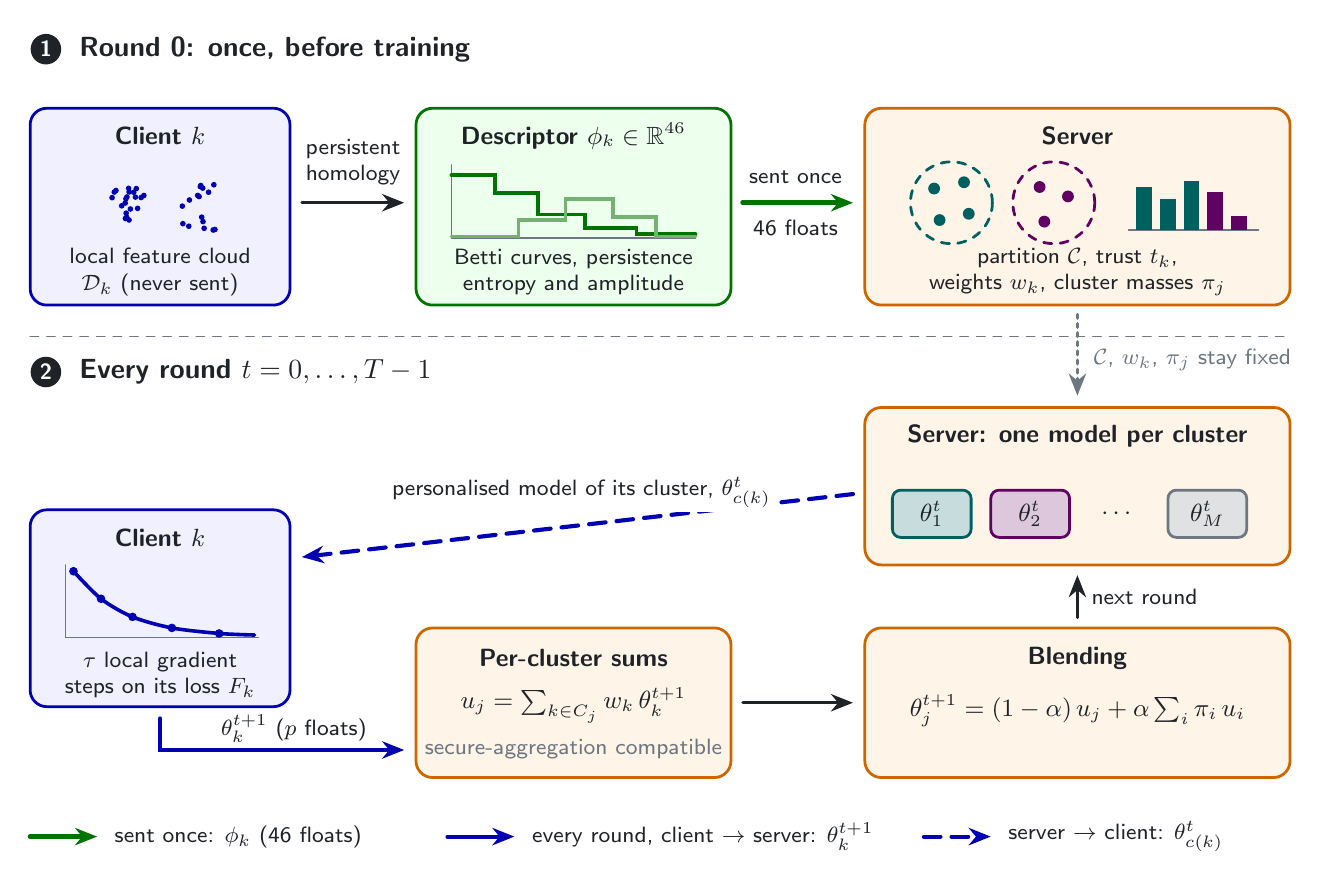
\begin{tikzpicture}[color=fg, font=\sffamily\small, line cap=round,
  >={Stealth[length=2.8mm,width=2.2mm]},
  box/.style={rounded corners=6pt, line width=1pt},
  head/.style={font=\sffamily\bfseries\small, text=fg},
  note/.style={font=\sffamily\footnotesize, text=fg, align=center},
  lab/.style={font=\sffamily\footnotesize, text=fg, fill=bg, inner sep=1.5pt, align=center},
  num/.style={circle, fill=fg, text=bg, inner sep=1.4pt, font=\sffamily\bfseries\footnotesize}]

% ============================ panel 1: round 0 ============================
\node[num] at (0.2,9.25) {1};
\node[anchor=west, font=\sffamily\bfseries\normalsize, text=fg] at (0.5,9.25) {Round 0: once, before training};

% client
\draw[box, draw=cl, fill=clfill] (0,6.0) rectangle (3.3,8.5);
\node[head] at (1.65,8.15) {Client $k$};
\pgfmathsetseed{11}
\foreach \i in {1,...,20} {\fill[cl] ({1.15+0.30*rand},{7.30+0.26*rand}) circle (0.036);}
\foreach \i in {1,...,16} {\fill[cl] ({2.15+0.22*rand},{7.25+0.32*rand}) circle (0.036);}
\node[note] at (1.65,6.42) {local feature cloud\\$\mathcal D_k$ (never sent)};

\draw[->, line width=1.1pt] (3.45,7.3) -- (4.75,7.3);
\node[note] at (4.1,7.82) {persistent\\homology};

% descriptor
\draw[box, draw=ds, fill=dsfill] (4.9,6.0) rectangle (8.9,8.5);
\node[head] at (6.9,8.15) {Descriptor $\phi_k\in\mathbb{R}^{46}$};
\draw[muted, line width=0.6pt] (5.35,6.85) -- (8.45,6.85);
\draw[muted, line width=0.6pt] (5.35,6.85) -- (5.35,7.78);
\draw[ds, line width=1.3pt] (5.35,7.65) -- (5.9,7.65) -- (5.9,7.42) -- (6.45,7.42) -- (6.45,7.15) -- (7.05,7.15)
      -- (7.05,6.98) -- (7.7,6.98) -- (7.7,6.9) -- (8.45,6.9);
\draw[ds!55!bg, line width=1.3pt] (5.35,6.87) -- (6.2,6.87) -- (6.2,7.08) -- (6.8,7.08) -- (6.8,7.35) -- (7.4,7.35)
      -- (7.4,7.12) -- (7.95,7.12) -- (7.95,6.87) -- (8.45,6.87);
\node[note] at (6.9,6.42) {Betti curves, persistence\\entropy and amplitude};

\draw[->, line width=1.8pt, draw=ds] (9.05,7.3) -- (10.45,7.3);
\node[lab] at (9.72,7.62) {sent once};
\node[lab] at (9.72,6.98) {46 floats};

% server structure
\draw[box, draw=sv, fill=svfill] (10.6,6.0) rectangle (16.0,8.5);
\node[head] at (13.3,8.15) {Server};
\draw[ca, dashed, line width=1pt] (11.7,7.3) circle (0.52);
\draw[cb, dashed, line width=1pt] (13.0,7.3) circle (0.52);
\foreach \p in {(11.48,7.48),(11.86,7.56),(11.55,7.08),(11.92,7.16)} \fill[ca] \p circle (0.075);
\foreach \p in {(12.82,7.5),(13.18,7.38),(12.88,7.06)} \fill[cb] \p circle (0.075);
\draw[muted, line width=0.6pt] (13.95,6.95) -- (15.6,6.95);
\foreach \x/\h/\c in {14.15/0.55/ca, 14.45/0.40/ca, 14.75/0.62/ca, 15.05/0.48/cb, 15.35/0.18/cb}
  \fill[\c] (\x-0.1,6.95) rectangle (\x+0.1,6.95+\h);
\node[note] at (13.3,6.42) {partition $\mathcal C$, trust $t_k$,\\weights $w_k$, cluster masses $\pi_j$};

% ============================ separator ============================
\draw[muted, dashed, line width=0.6pt] (0,5.6) -- (16,5.6);
\draw[->, muted, dotted, line width=1.3pt] (13.3,5.88) -- (13.3,4.85);
\node[lab, anchor=west, text=muted] at (13.45,5.3) {$\mathcal C$, $w_k$, $\pi_j$ stay fixed};

% ============================ panel 2: every round ============================
\node[num] at (0.2,5.15) {2};
\node[anchor=west, font=\sffamily\bfseries\normalsize, text=fg] at (0.5,5.15) {Every round $t=0,\dots,T-1$};

% server models
\draw[box, draw=sv, fill=svfill] (10.6,2.7) rectangle (16.0,4.7);
\node[head] at (13.3,4.33) {Server: one model per cluster};
\foreach \x/\c/\t in {11.45/ca/1, 12.7/cb/2, 14.95/muted/M}
  {\draw[\c, fill=\c!22!bg, rounded corners=3pt, line width=1pt] (\x-0.5,3.05) rectangle (\x+0.5,3.65);
   \node[text=fg] at (\x,3.35) {$\theta^{t}_{\t}$};}
\node[text=fg] at (13.82,3.35) {$\cdots$};

% client training
\draw[box, draw=cl, fill=clfill] (0,0.9) rectangle (3.3,3.4);
\node[head] at (1.65,3.05) {Client $k$};
\draw[muted, line width=0.6pt] (0.45,1.78) -- (2.9,1.78);
\draw[muted, line width=0.6pt] (0.45,1.78) -- (0.45,2.7);
\draw[cl, line width=1.3pt] plot[smooth] coordinates {(0.55,2.62) (0.9,2.27) (1.3,2.04) (1.8,1.9) (2.4,1.83) (2.85,1.81)};
\foreach \p in {(0.55,2.62),(0.9,2.27),(1.3,2.04),(1.8,1.9),(2.4,1.83)} \fill[cl] \p circle (0.055);
\node[note] at (1.65,1.3) {$\tau$ local gradient\\steps on its loss $F_k$};

% broadcast (dashed) and upload (solid)
\draw[->, line width=1.5pt, draw=cl, dash pattern=on 6pt off 4pt] (10.45,3.6) -- (3.45,2.8);
\node[lab] at (7.0,3.62) {personalised model of its cluster, $\theta^{t}_{c(k)}$};
\draw[->, line width=1.5pt, draw=cl] (1.65,0.75) |- (4.75,0.35);
\node[lab] at (3.35,0.62) {$\theta^{t+1}_k$ ($p$ floats)};

% aggregation and blending
\draw[box, draw=sv, fill=svfill] (4.9,0) rectangle (8.9,1.9);
\node[head] at (6.9,1.52) {Per-cluster sums};
\node[text=fg] at (6.9,0.92) {$u_j=\sum_{k\in C_j} w_k\,\theta^{t+1}_k$};
\node[note, text=muted] at (6.9,0.36) {secure-aggregation compatible};
\draw[->, line width=1.1pt] (9.05,0.95) -- (10.45,0.95);
\draw[box, draw=sv, fill=svfill] (10.6,0) rectangle (16.0,1.9);
\node[head] at (13.3,1.52) {Blending};
\node[text=fg] at (13.3,0.85) {$\theta^{t+1}_j=(1-\alpha)\,u_j+\alpha\sum_i\pi_i\,u_i$};
\draw[->, line width=1.1pt] (13.3,2.03) -- (13.3,2.57);
\node[lab, anchor=west] at (13.42,2.3) {next round};

% ============================ legend ============================
\draw[->, line width=1.8pt, draw=ds] (0,-0.75) -- (0.85,-0.75);
\node[anchor=west, font=\sffamily\footnotesize] at (0.95,-0.75) {sent once: $\phi_k$ (46 floats)};
\draw[->, line width=1.5pt, draw=cl] (5.3,-0.75) -- (6.15,-0.75);
\node[anchor=west, font=\sffamily\footnotesize] at (6.25,-0.75) {every round, client $\to$ server: $\theta^{t+1}_k$};
\draw[->, line width=1.5pt, draw=cl, dash pattern=on 6pt off 4pt] (11.35,-0.75) -- (12.2,-0.75);
\node[anchor=west, font=\sffamily\footnotesize] at (12.3,-0.75) {server $\to$ client: $\theta^{t}_{c(k)}$};
\end{tikzpicture}
\end{document}
"
%   pdflatex -jobname=ptopofl_protocol_dark  "\def\isdark{1}% pTopoFL protocol figure for the README.  Build:
%   pdflatex -jobname=ptopofl_protocol_light "\def\isdark{0}\input{ptopofl_protocol}"
%   pdflatex -jobname=ptopofl_protocol_dark  "\def\isdark{1}\input{ptopofl_protocol}"
%   pdftocairo -svg <name>.pdf <name>.svg   (and pdftoppm -png -r 300 -singlefile <name>.pdf <name>)
\documentclass[border=14pt]{standalone}
\usepackage{amsmath,amssymb}
\usepackage[scaled=0.92]{helvet}
\renewcommand{\familydefault}{\sfdefault}
\usepackage{tikz}
\usetikzlibrary{arrows.meta,calc}
\providecommand{\isdark}{0}
\ifnum\isdark=1
  \definecolor{bg}{HTML}{0D1117}\definecolor{fg}{HTML}{E6EDF3}\definecolor{muted}{HTML}{8B949E}
  \colorlet{cl}{blue!35!white}\colorlet{clfill}{blue!16!bg}
  \colorlet{ds}{green!65!white}\colorlet{dsfill}{green!12!bg}
  \colorlet{sv}{orange!80!white}\colorlet{svfill}{orange!13!bg}
  \colorlet{ca}{cyan!75!white}\colorlet{cb}{magenta!55!white}
\else
  \definecolor{bg}{HTML}{FFFFFF}\definecolor{fg}{HTML}{1F2328}\definecolor{muted}{HTML}{6E7781}
  \colorlet{cl}{blue!70!black}\colorlet{clfill}{blue!6}
  \colorlet{ds}{green!45!black}\colorlet{dsfill}{green!7}
  \colorlet{sv}{orange!80!black}\colorlet{svfill}{orange!9}
  \colorlet{ca}{teal!75!black}\colorlet{cb}{violet!75!black}
\fi
\pagecolor{bg}
\begin{document}
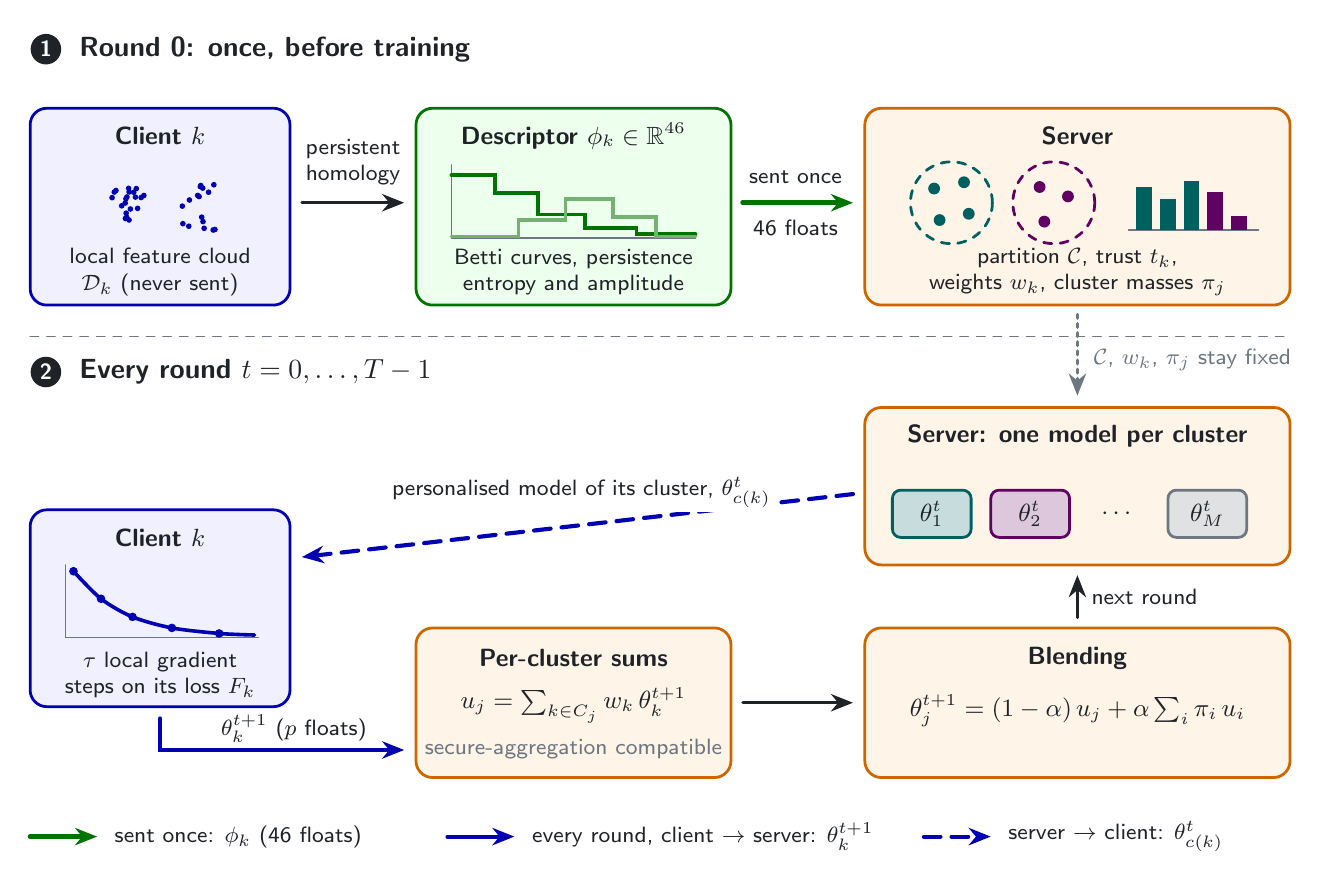
\begin{tikzpicture}[color=fg, font=\sffamily\small, line cap=round,
  >={Stealth[length=2.8mm,width=2.2mm]},
  box/.style={rounded corners=6pt, line width=1pt},
  head/.style={font=\sffamily\bfseries\small, text=fg},
  note/.style={font=\sffamily\footnotesize, text=fg, align=center},
  lab/.style={font=\sffamily\footnotesize, text=fg, fill=bg, inner sep=1.5pt, align=center},
  num/.style={circle, fill=fg, text=bg, inner sep=1.4pt, font=\sffamily\bfseries\footnotesize}]

% ============================ panel 1: round 0 ============================
\node[num] at (0.2,9.25) {1};
\node[anchor=west, font=\sffamily\bfseries\normalsize, text=fg] at (0.5,9.25) {Round 0: once, before training};

% client
\draw[box, draw=cl, fill=clfill] (0,6.0) rectangle (3.3,8.5);
\node[head] at (1.65,8.15) {Client $k$};
\pgfmathsetseed{11}
\foreach \i in {1,...,20} {\fill[cl] ({1.15+0.30*rand},{7.30+0.26*rand}) circle (0.036);}
\foreach \i in {1,...,16} {\fill[cl] ({2.15+0.22*rand},{7.25+0.32*rand}) circle (0.036);}
\node[note] at (1.65,6.42) {local feature cloud\\$\mathcal D_k$ (never sent)};

\draw[->, line width=1.1pt] (3.45,7.3) -- (4.75,7.3);
\node[note] at (4.1,7.82) {persistent\\homology};

% descriptor
\draw[box, draw=ds, fill=dsfill] (4.9,6.0) rectangle (8.9,8.5);
\node[head] at (6.9,8.15) {Descriptor $\phi_k\in\mathbb{R}^{46}$};
\draw[muted, line width=0.6pt] (5.35,6.85) -- (8.45,6.85);
\draw[muted, line width=0.6pt] (5.35,6.85) -- (5.35,7.78);
\draw[ds, line width=1.3pt] (5.35,7.65) -- (5.9,7.65) -- (5.9,7.42) -- (6.45,7.42) -- (6.45,7.15) -- (7.05,7.15)
      -- (7.05,6.98) -- (7.7,6.98) -- (7.7,6.9) -- (8.45,6.9);
\draw[ds!55!bg, line width=1.3pt] (5.35,6.87) -- (6.2,6.87) -- (6.2,7.08) -- (6.8,7.08) -- (6.8,7.35) -- (7.4,7.35)
      -- (7.4,7.12) -- (7.95,7.12) -- (7.95,6.87) -- (8.45,6.87);
\node[note] at (6.9,6.42) {Betti curves, persistence\\entropy and amplitude};

\draw[->, line width=1.8pt, draw=ds] (9.05,7.3) -- (10.45,7.3);
\node[lab] at (9.72,7.62) {sent once};
\node[lab] at (9.72,6.98) {46 floats};

% server structure
\draw[box, draw=sv, fill=svfill] (10.6,6.0) rectangle (16.0,8.5);
\node[head] at (13.3,8.15) {Server};
\draw[ca, dashed, line width=1pt] (11.7,7.3) circle (0.52);
\draw[cb, dashed, line width=1pt] (13.0,7.3) circle (0.52);
\foreach \p in {(11.48,7.48),(11.86,7.56),(11.55,7.08),(11.92,7.16)} \fill[ca] \p circle (0.075);
\foreach \p in {(12.82,7.5),(13.18,7.38),(12.88,7.06)} \fill[cb] \p circle (0.075);
\draw[muted, line width=0.6pt] (13.95,6.95) -- (15.6,6.95);
\foreach \x/\h/\c in {14.15/0.55/ca, 14.45/0.40/ca, 14.75/0.62/ca, 15.05/0.48/cb, 15.35/0.18/cb}
  \fill[\c] (\x-0.1,6.95) rectangle (\x+0.1,6.95+\h);
\node[note] at (13.3,6.42) {partition $\mathcal C$, trust $t_k$,\\weights $w_k$, cluster masses $\pi_j$};

% ============================ separator ============================
\draw[muted, dashed, line width=0.6pt] (0,5.6) -- (16,5.6);
\draw[->, muted, dotted, line width=1.3pt] (13.3,5.88) -- (13.3,4.85);
\node[lab, anchor=west, text=muted] at (13.45,5.3) {$\mathcal C$, $w_k$, $\pi_j$ stay fixed};

% ============================ panel 2: every round ============================
\node[num] at (0.2,5.15) {2};
\node[anchor=west, font=\sffamily\bfseries\normalsize, text=fg] at (0.5,5.15) {Every round $t=0,\dots,T-1$};

% server models
\draw[box, draw=sv, fill=svfill] (10.6,2.7) rectangle (16.0,4.7);
\node[head] at (13.3,4.33) {Server: one model per cluster};
\foreach \x/\c/\t in {11.45/ca/1, 12.7/cb/2, 14.95/muted/M}
  {\draw[\c, fill=\c!22!bg, rounded corners=3pt, line width=1pt] (\x-0.5,3.05) rectangle (\x+0.5,3.65);
   \node[text=fg] at (\x,3.35) {$\theta^{t}_{\t}$};}
\node[text=fg] at (13.82,3.35) {$\cdots$};

% client training
\draw[box, draw=cl, fill=clfill] (0,0.9) rectangle (3.3,3.4);
\node[head] at (1.65,3.05) {Client $k$};
\draw[muted, line width=0.6pt] (0.45,1.78) -- (2.9,1.78);
\draw[muted, line width=0.6pt] (0.45,1.78) -- (0.45,2.7);
\draw[cl, line width=1.3pt] plot[smooth] coordinates {(0.55,2.62) (0.9,2.27) (1.3,2.04) (1.8,1.9) (2.4,1.83) (2.85,1.81)};
\foreach \p in {(0.55,2.62),(0.9,2.27),(1.3,2.04),(1.8,1.9),(2.4,1.83)} \fill[cl] \p circle (0.055);
\node[note] at (1.65,1.3) {$\tau$ local gradient\\steps on its loss $F_k$};

% broadcast (dashed) and upload (solid)
\draw[->, line width=1.5pt, draw=cl, dash pattern=on 6pt off 4pt] (10.45,3.6) -- (3.45,2.8);
\node[lab] at (7.0,3.62) {personalised model of its cluster, $\theta^{t}_{c(k)}$};
\draw[->, line width=1.5pt, draw=cl] (1.65,0.75) |- (4.75,0.35);
\node[lab] at (3.35,0.62) {$\theta^{t+1}_k$ ($p$ floats)};

% aggregation and blending
\draw[box, draw=sv, fill=svfill] (4.9,0) rectangle (8.9,1.9);
\node[head] at (6.9,1.52) {Per-cluster sums};
\node[text=fg] at (6.9,0.92) {$u_j=\sum_{k\in C_j} w_k\,\theta^{t+1}_k$};
\node[note, text=muted] at (6.9,0.36) {secure-aggregation compatible};
\draw[->, line width=1.1pt] (9.05,0.95) -- (10.45,0.95);
\draw[box, draw=sv, fill=svfill] (10.6,0) rectangle (16.0,1.9);
\node[head] at (13.3,1.52) {Blending};
\node[text=fg] at (13.3,0.85) {$\theta^{t+1}_j=(1-\alpha)\,u_j+\alpha\sum_i\pi_i\,u_i$};
\draw[->, line width=1.1pt] (13.3,2.03) -- (13.3,2.57);
\node[lab, anchor=west] at (13.42,2.3) {next round};

% ============================ legend ============================
\draw[->, line width=1.8pt, draw=ds] (0,-0.75) -- (0.85,-0.75);
\node[anchor=west, font=\sffamily\footnotesize] at (0.95,-0.75) {sent once: $\phi_k$ (46 floats)};
\draw[->, line width=1.5pt, draw=cl] (5.3,-0.75) -- (6.15,-0.75);
\node[anchor=west, font=\sffamily\footnotesize] at (6.25,-0.75) {every round, client $\to$ server: $\theta^{t+1}_k$};
\draw[->, line width=1.5pt, draw=cl, dash pattern=on 6pt off 4pt] (11.35,-0.75) -- (12.2,-0.75);
\node[anchor=west, font=\sffamily\footnotesize] at (12.3,-0.75) {server $\to$ client: $\theta^{t}_{c(k)}$};
\end{tikzpicture}
\end{document}
"
%   pdftocairo -svg <name>.pdf <name>.svg   (and pdftoppm -png -r 300 -singlefile <name>.pdf <name>)
\documentclass[border=14pt]{standalone}
\usepackage{amsmath,amssymb}
\usepackage[scaled=0.92]{helvet}
\renewcommand{\familydefault}{\sfdefault}
\usepackage{tikz}
\usetikzlibrary{arrows.meta,calc}
\providecommand{\isdark}{0}
\ifnum\isdark=1
  \definecolor{bg}{HTML}{0D1117}\definecolor{fg}{HTML}{E6EDF3}\definecolor{muted}{HTML}{8B949E}
  \colorlet{cl}{blue!35!white}\colorlet{clfill}{blue!16!bg}
  \colorlet{ds}{green!65!white}\colorlet{dsfill}{green!12!bg}
  \colorlet{sv}{orange!80!white}\colorlet{svfill}{orange!13!bg}
  \colorlet{ca}{cyan!75!white}\colorlet{cb}{magenta!55!white}
\else
  \definecolor{bg}{HTML}{FFFFFF}\definecolor{fg}{HTML}{1F2328}\definecolor{muted}{HTML}{6E7781}
  \colorlet{cl}{blue!70!black}\colorlet{clfill}{blue!6}
  \colorlet{ds}{green!45!black}\colorlet{dsfill}{green!7}
  \colorlet{sv}{orange!80!black}\colorlet{svfill}{orange!9}
  \colorlet{ca}{teal!75!black}\colorlet{cb}{violet!75!black}
\fi
\pagecolor{bg}
\begin{document}
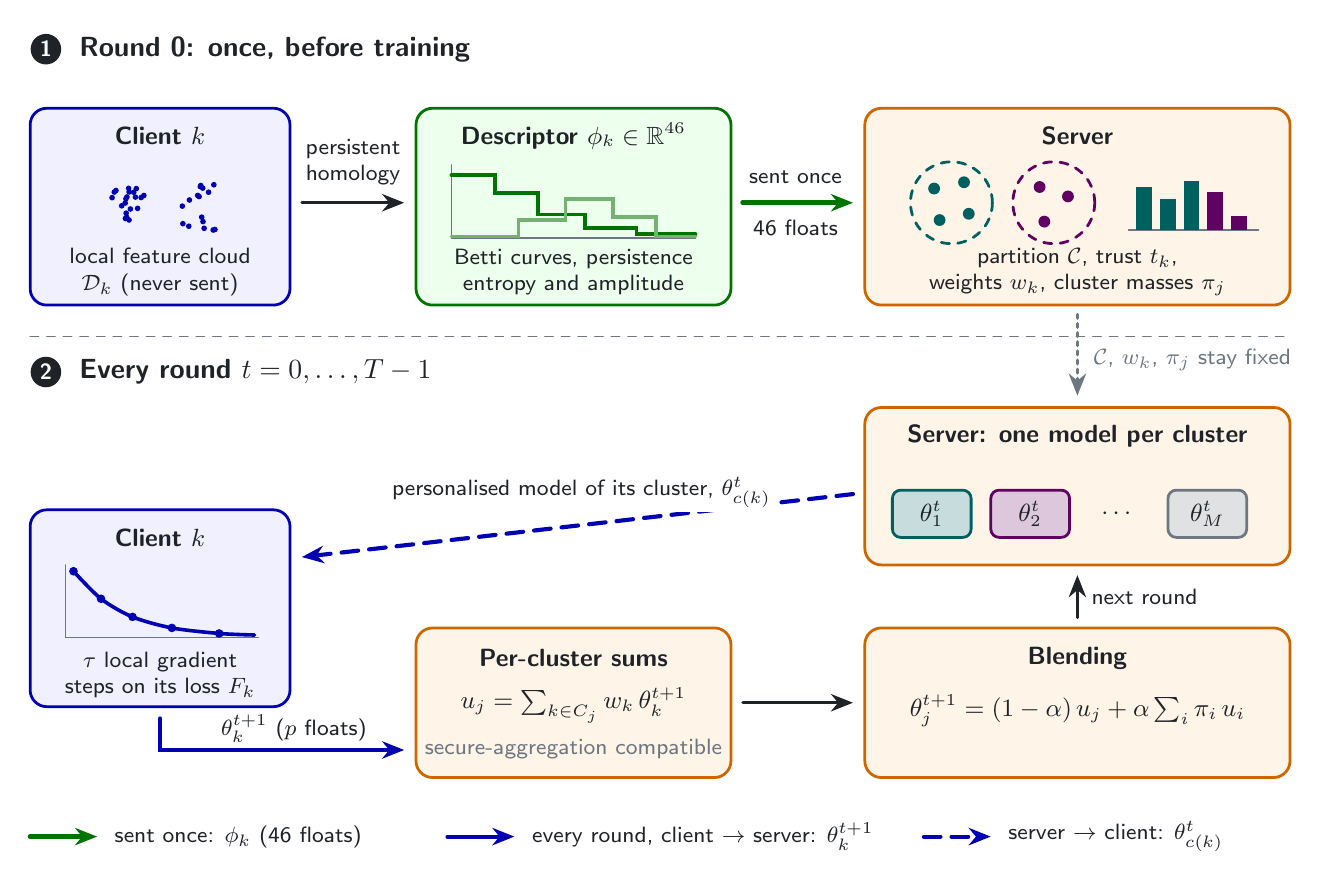
\begin{tikzpicture}[color=fg, font=\sffamily\small, line cap=round,
  >={Stealth[length=2.8mm,width=2.2mm]},
  box/.style={rounded corners=6pt, line width=1pt},
  head/.style={font=\sffamily\bfseries\small, text=fg},
  note/.style={font=\sffamily\footnotesize, text=fg, align=center},
  lab/.style={font=\sffamily\footnotesize, text=fg, fill=bg, inner sep=1.5pt, align=center},
  num/.style={circle, fill=fg, text=bg, inner sep=1.4pt, font=\sffamily\bfseries\footnotesize}]

% ============================ panel 1: round 0 ============================
\node[num] at (0.2,9.25) {1};
\node[anchor=west, font=\sffamily\bfseries\normalsize, text=fg] at (0.5,9.25) {Round 0: once, before training};

% client
\draw[box, draw=cl, fill=clfill] (0,6.0) rectangle (3.3,8.5);
\node[head] at (1.65,8.15) {Client $k$};
\pgfmathsetseed{11}
\foreach \i in {1,...,20} {\fill[cl] ({1.15+0.30*rand},{7.30+0.26*rand}) circle (0.036);}
\foreach \i in {1,...,16} {\fill[cl] ({2.15+0.22*rand},{7.25+0.32*rand}) circle (0.036);}
\node[note] at (1.65,6.42) {local feature cloud\\$\mathcal D_k$ (never sent)};

\draw[->, line width=1.1pt] (3.45,7.3) -- (4.75,7.3);
\node[note] at (4.1,7.82) {persistent\\homology};

% descriptor
\draw[box, draw=ds, fill=dsfill] (4.9,6.0) rectangle (8.9,8.5);
\node[head] at (6.9,8.15) {Descriptor $\phi_k\in\mathbb{R}^{46}$};
\draw[muted, line width=0.6pt] (5.35,6.85) -- (8.45,6.85);
\draw[muted, line width=0.6pt] (5.35,6.85) -- (5.35,7.78);
\draw[ds, line width=1.3pt] (5.35,7.65) -- (5.9,7.65) -- (5.9,7.42) -- (6.45,7.42) -- (6.45,7.15) -- (7.05,7.15)
      -- (7.05,6.98) -- (7.7,6.98) -- (7.7,6.9) -- (8.45,6.9);
\draw[ds!55!bg, line width=1.3pt] (5.35,6.87) -- (6.2,6.87) -- (6.2,7.08) -- (6.8,7.08) -- (6.8,7.35) -- (7.4,7.35)
      -- (7.4,7.12) -- (7.95,7.12) -- (7.95,6.87) -- (8.45,6.87);
\node[note] at (6.9,6.42) {Betti curves, persistence\\entropy and amplitude};

\draw[->, line width=1.8pt, draw=ds] (9.05,7.3) -- (10.45,7.3);
\node[lab] at (9.72,7.62) {sent once};
\node[lab] at (9.72,6.98) {46 floats};

% server structure
\draw[box, draw=sv, fill=svfill] (10.6,6.0) rectangle (16.0,8.5);
\node[head] at (13.3,8.15) {Server};
\draw[ca, dashed, line width=1pt] (11.7,7.3) circle (0.52);
\draw[cb, dashed, line width=1pt] (13.0,7.3) circle (0.52);
\foreach \p in {(11.48,7.48),(11.86,7.56),(11.55,7.08),(11.92,7.16)} \fill[ca] \p circle (0.075);
\foreach \p in {(12.82,7.5),(13.18,7.38),(12.88,7.06)} \fill[cb] \p circle (0.075);
\draw[muted, line width=0.6pt] (13.95,6.95) -- (15.6,6.95);
\foreach \x/\h/\c in {14.15/0.55/ca, 14.45/0.40/ca, 14.75/0.62/ca, 15.05/0.48/cb, 15.35/0.18/cb}
  \fill[\c] (\x-0.1,6.95) rectangle (\x+0.1,6.95+\h);
\node[note] at (13.3,6.42) {partition $\mathcal C$, trust $t_k$,\\weights $w_k$, cluster masses $\pi_j$};

% ============================ separator ============================
\draw[muted, dashed, line width=0.6pt] (0,5.6) -- (16,5.6);
\draw[->, muted, dotted, line width=1.3pt] (13.3,5.88) -- (13.3,4.85);
\node[lab, anchor=west, text=muted] at (13.45,5.3) {$\mathcal C$, $w_k$, $\pi_j$ stay fixed};

% ============================ panel 2: every round ============================
\node[num] at (0.2,5.15) {2};
\node[anchor=west, font=\sffamily\bfseries\normalsize, text=fg] at (0.5,5.15) {Every round $t=0,\dots,T-1$};

% server models
\draw[box, draw=sv, fill=svfill] (10.6,2.7) rectangle (16.0,4.7);
\node[head] at (13.3,4.33) {Server: one model per cluster};
\foreach \x/\c/\t in {11.45/ca/1, 12.7/cb/2, 14.95/muted/M}
  {\draw[\c, fill=\c!22!bg, rounded corners=3pt, line width=1pt] (\x-0.5,3.05) rectangle (\x+0.5,3.65);
   \node[text=fg] at (\x,3.35) {$\theta^{t}_{\t}$};}
\node[text=fg] at (13.82,3.35) {$\cdots$};

% client training
\draw[box, draw=cl, fill=clfill] (0,0.9) rectangle (3.3,3.4);
\node[head] at (1.65,3.05) {Client $k$};
\draw[muted, line width=0.6pt] (0.45,1.78) -- (2.9,1.78);
\draw[muted, line width=0.6pt] (0.45,1.78) -- (0.45,2.7);
\draw[cl, line width=1.3pt] plot[smooth] coordinates {(0.55,2.62) (0.9,2.27) (1.3,2.04) (1.8,1.9) (2.4,1.83) (2.85,1.81)};
\foreach \p in {(0.55,2.62),(0.9,2.27),(1.3,2.04),(1.8,1.9),(2.4,1.83)} \fill[cl] \p circle (0.055);
\node[note] at (1.65,1.3) {$\tau$ local gradient\\steps on its loss $F_k$};

% broadcast (dashed) and upload (solid)
\draw[->, line width=1.5pt, draw=cl, dash pattern=on 6pt off 4pt] (10.45,3.6) -- (3.45,2.8);
\node[lab] at (7.0,3.62) {personalised model of its cluster, $\theta^{t}_{c(k)}$};
\draw[->, line width=1.5pt, draw=cl] (1.65,0.75) |- (4.75,0.35);
\node[lab] at (3.35,0.62) {$\theta^{t+1}_k$ ($p$ floats)};

% aggregation and blending
\draw[box, draw=sv, fill=svfill] (4.9,0) rectangle (8.9,1.9);
\node[head] at (6.9,1.52) {Per-cluster sums};
\node[text=fg] at (6.9,0.92) {$u_j=\sum_{k\in C_j} w_k\,\theta^{t+1}_k$};
\node[note, text=muted] at (6.9,0.36) {secure-aggregation compatible};
\draw[->, line width=1.1pt] (9.05,0.95) -- (10.45,0.95);
\draw[box, draw=sv, fill=svfill] (10.6,0) rectangle (16.0,1.9);
\node[head] at (13.3,1.52) {Blending};
\node[text=fg] at (13.3,0.85) {$\theta^{t+1}_j=(1-\alpha)\,u_j+\alpha\sum_i\pi_i\,u_i$};
\draw[->, line width=1.1pt] (13.3,2.03) -- (13.3,2.57);
\node[lab, anchor=west] at (13.42,2.3) {next round};

% ============================ legend ============================
\draw[->, line width=1.8pt, draw=ds] (0,-0.75) -- (0.85,-0.75);
\node[anchor=west, font=\sffamily\footnotesize] at (0.95,-0.75) {sent once: $\phi_k$ (46 floats)};
\draw[->, line width=1.5pt, draw=cl] (5.3,-0.75) -- (6.15,-0.75);
\node[anchor=west, font=\sffamily\footnotesize] at (6.25,-0.75) {every round, client $\to$ server: $\theta^{t+1}_k$};
\draw[->, line width=1.5pt, draw=cl, dash pattern=on 6pt off 4pt] (11.35,-0.75) -- (12.2,-0.75);
\node[anchor=west, font=\sffamily\footnotesize] at (12.3,-0.75) {server $\to$ client: $\theta^{t}_{c(k)}$};
\end{tikzpicture}
\end{document}
"
%   pdflatex -jobname=ptopofl_protocol_dark  "\def\isdark{1}% pTopoFL protocol figure for the README.  Build:
%   pdflatex -jobname=ptopofl_protocol_light "\def\isdark{0}% pTopoFL protocol figure for the README.  Build:
%   pdflatex -jobname=ptopofl_protocol_light "\def\isdark{0}\input{ptopofl_protocol}"
%   pdflatex -jobname=ptopofl_protocol_dark  "\def\isdark{1}\input{ptopofl_protocol}"
%   pdftocairo -svg <name>.pdf <name>.svg   (and pdftoppm -png -r 300 -singlefile <name>.pdf <name>)
\documentclass[border=14pt]{standalone}
\usepackage{amsmath,amssymb}
\usepackage[scaled=0.92]{helvet}
\renewcommand{\familydefault}{\sfdefault}
\usepackage{tikz}
\usetikzlibrary{arrows.meta,calc}
\providecommand{\isdark}{0}
\ifnum\isdark=1
  \definecolor{bg}{HTML}{0D1117}\definecolor{fg}{HTML}{E6EDF3}\definecolor{muted}{HTML}{8B949E}
  \colorlet{cl}{blue!35!white}\colorlet{clfill}{blue!16!bg}
  \colorlet{ds}{green!65!white}\colorlet{dsfill}{green!12!bg}
  \colorlet{sv}{orange!80!white}\colorlet{svfill}{orange!13!bg}
  \colorlet{ca}{cyan!75!white}\colorlet{cb}{magenta!55!white}
\else
  \definecolor{bg}{HTML}{FFFFFF}\definecolor{fg}{HTML}{1F2328}\definecolor{muted}{HTML}{6E7781}
  \colorlet{cl}{blue!70!black}\colorlet{clfill}{blue!6}
  \colorlet{ds}{green!45!black}\colorlet{dsfill}{green!7}
  \colorlet{sv}{orange!80!black}\colorlet{svfill}{orange!9}
  \colorlet{ca}{teal!75!black}\colorlet{cb}{violet!75!black}
\fi
\pagecolor{bg}
\begin{document}
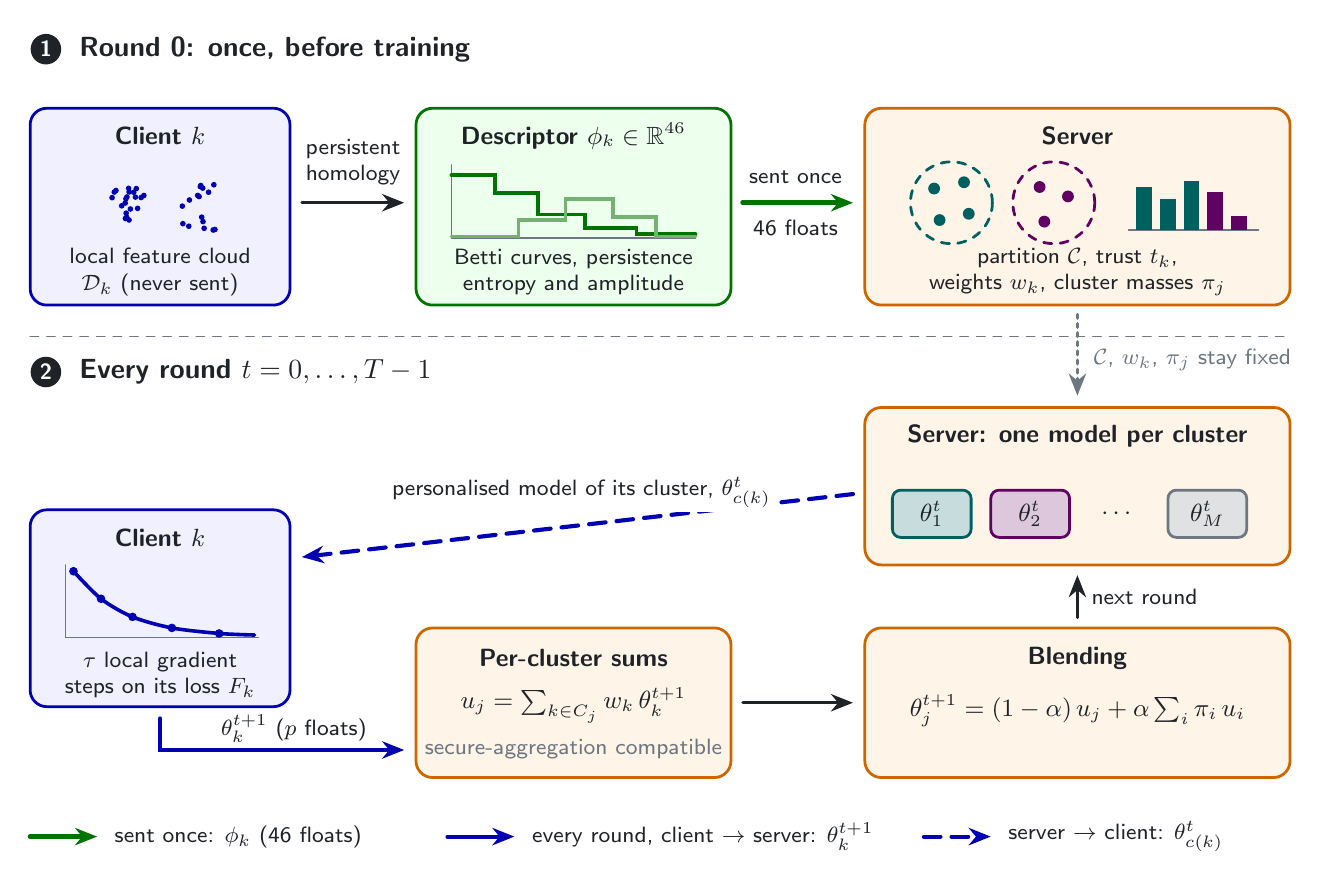
\begin{tikzpicture}[color=fg, font=\sffamily\small, line cap=round,
  >={Stealth[length=2.8mm,width=2.2mm]},
  box/.style={rounded corners=6pt, line width=1pt},
  head/.style={font=\sffamily\bfseries\small, text=fg},
  note/.style={font=\sffamily\footnotesize, text=fg, align=center},
  lab/.style={font=\sffamily\footnotesize, text=fg, fill=bg, inner sep=1.5pt, align=center},
  num/.style={circle, fill=fg, text=bg, inner sep=1.4pt, font=\sffamily\bfseries\footnotesize}]

% ============================ panel 1: round 0 ============================
\node[num] at (0.2,9.25) {1};
\node[anchor=west, font=\sffamily\bfseries\normalsize, text=fg] at (0.5,9.25) {Round 0: once, before training};

% client
\draw[box, draw=cl, fill=clfill] (0,6.0) rectangle (3.3,8.5);
\node[head] at (1.65,8.15) {Client $k$};
\pgfmathsetseed{11}
\foreach \i in {1,...,20} {\fill[cl] ({1.15+0.30*rand},{7.30+0.26*rand}) circle (0.036);}
\foreach \i in {1,...,16} {\fill[cl] ({2.15+0.22*rand},{7.25+0.32*rand}) circle (0.036);}
\node[note] at (1.65,6.42) {local feature cloud\\$\mathcal D_k$ (never sent)};

\draw[->, line width=1.1pt] (3.45,7.3) -- (4.75,7.3);
\node[note] at (4.1,7.82) {persistent\\homology};

% descriptor
\draw[box, draw=ds, fill=dsfill] (4.9,6.0) rectangle (8.9,8.5);
\node[head] at (6.9,8.15) {Descriptor $\phi_k\in\mathbb{R}^{46}$};
\draw[muted, line width=0.6pt] (5.35,6.85) -- (8.45,6.85);
\draw[muted, line width=0.6pt] (5.35,6.85) -- (5.35,7.78);
\draw[ds, line width=1.3pt] (5.35,7.65) -- (5.9,7.65) -- (5.9,7.42) -- (6.45,7.42) -- (6.45,7.15) -- (7.05,7.15)
      -- (7.05,6.98) -- (7.7,6.98) -- (7.7,6.9) -- (8.45,6.9);
\draw[ds!55!bg, line width=1.3pt] (5.35,6.87) -- (6.2,6.87) -- (6.2,7.08) -- (6.8,7.08) -- (6.8,7.35) -- (7.4,7.35)
      -- (7.4,7.12) -- (7.95,7.12) -- (7.95,6.87) -- (8.45,6.87);
\node[note] at (6.9,6.42) {Betti curves, persistence\\entropy and amplitude};

\draw[->, line width=1.8pt, draw=ds] (9.05,7.3) -- (10.45,7.3);
\node[lab] at (9.72,7.62) {sent once};
\node[lab] at (9.72,6.98) {46 floats};

% server structure
\draw[box, draw=sv, fill=svfill] (10.6,6.0) rectangle (16.0,8.5);
\node[head] at (13.3,8.15) {Server};
\draw[ca, dashed, line width=1pt] (11.7,7.3) circle (0.52);
\draw[cb, dashed, line width=1pt] (13.0,7.3) circle (0.52);
\foreach \p in {(11.48,7.48),(11.86,7.56),(11.55,7.08),(11.92,7.16)} \fill[ca] \p circle (0.075);
\foreach \p in {(12.82,7.5),(13.18,7.38),(12.88,7.06)} \fill[cb] \p circle (0.075);
\draw[muted, line width=0.6pt] (13.95,6.95) -- (15.6,6.95);
\foreach \x/\h/\c in {14.15/0.55/ca, 14.45/0.40/ca, 14.75/0.62/ca, 15.05/0.48/cb, 15.35/0.18/cb}
  \fill[\c] (\x-0.1,6.95) rectangle (\x+0.1,6.95+\h);
\node[note] at (13.3,6.42) {partition $\mathcal C$, trust $t_k$,\\weights $w_k$, cluster masses $\pi_j$};

% ============================ separator ============================
\draw[muted, dashed, line width=0.6pt] (0,5.6) -- (16,5.6);
\draw[->, muted, dotted, line width=1.3pt] (13.3,5.88) -- (13.3,4.85);
\node[lab, anchor=west, text=muted] at (13.45,5.3) {$\mathcal C$, $w_k$, $\pi_j$ stay fixed};

% ============================ panel 2: every round ============================
\node[num] at (0.2,5.15) {2};
\node[anchor=west, font=\sffamily\bfseries\normalsize, text=fg] at (0.5,5.15) {Every round $t=0,\dots,T-1$};

% server models
\draw[box, draw=sv, fill=svfill] (10.6,2.7) rectangle (16.0,4.7);
\node[head] at (13.3,4.33) {Server: one model per cluster};
\foreach \x/\c/\t in {11.45/ca/1, 12.7/cb/2, 14.95/muted/M}
  {\draw[\c, fill=\c!22!bg, rounded corners=3pt, line width=1pt] (\x-0.5,3.05) rectangle (\x+0.5,3.65);
   \node[text=fg] at (\x,3.35) {$\theta^{t}_{\t}$};}
\node[text=fg] at (13.82,3.35) {$\cdots$};

% client training
\draw[box, draw=cl, fill=clfill] (0,0.9) rectangle (3.3,3.4);
\node[head] at (1.65,3.05) {Client $k$};
\draw[muted, line width=0.6pt] (0.45,1.78) -- (2.9,1.78);
\draw[muted, line width=0.6pt] (0.45,1.78) -- (0.45,2.7);
\draw[cl, line width=1.3pt] plot[smooth] coordinates {(0.55,2.62) (0.9,2.27) (1.3,2.04) (1.8,1.9) (2.4,1.83) (2.85,1.81)};
\foreach \p in {(0.55,2.62),(0.9,2.27),(1.3,2.04),(1.8,1.9),(2.4,1.83)} \fill[cl] \p circle (0.055);
\node[note] at (1.65,1.3) {$\tau$ local gradient\\steps on its loss $F_k$};

% broadcast (dashed) and upload (solid)
\draw[->, line width=1.5pt, draw=cl, dash pattern=on 6pt off 4pt] (10.45,3.6) -- (3.45,2.8);
\node[lab] at (7.0,3.62) {personalised model of its cluster, $\theta^{t}_{c(k)}$};
\draw[->, line width=1.5pt, draw=cl] (1.65,0.75) |- (4.75,0.35);
\node[lab] at (3.35,0.62) {$\theta^{t+1}_k$ ($p$ floats)};

% aggregation and blending
\draw[box, draw=sv, fill=svfill] (4.9,0) rectangle (8.9,1.9);
\node[head] at (6.9,1.52) {Per-cluster sums};
\node[text=fg] at (6.9,0.92) {$u_j=\sum_{k\in C_j} w_k\,\theta^{t+1}_k$};
\node[note, text=muted] at (6.9,0.36) {secure-aggregation compatible};
\draw[->, line width=1.1pt] (9.05,0.95) -- (10.45,0.95);
\draw[box, draw=sv, fill=svfill] (10.6,0) rectangle (16.0,1.9);
\node[head] at (13.3,1.52) {Blending};
\node[text=fg] at (13.3,0.85) {$\theta^{t+1}_j=(1-\alpha)\,u_j+\alpha\sum_i\pi_i\,u_i$};
\draw[->, line width=1.1pt] (13.3,2.03) -- (13.3,2.57);
\node[lab, anchor=west] at (13.42,2.3) {next round};

% ============================ legend ============================
\draw[->, line width=1.8pt, draw=ds] (0,-0.75) -- (0.85,-0.75);
\node[anchor=west, font=\sffamily\footnotesize] at (0.95,-0.75) {sent once: $\phi_k$ (46 floats)};
\draw[->, line width=1.5pt, draw=cl] (5.3,-0.75) -- (6.15,-0.75);
\node[anchor=west, font=\sffamily\footnotesize] at (6.25,-0.75) {every round, client $\to$ server: $\theta^{t+1}_k$};
\draw[->, line width=1.5pt, draw=cl, dash pattern=on 6pt off 4pt] (11.35,-0.75) -- (12.2,-0.75);
\node[anchor=west, font=\sffamily\footnotesize] at (12.3,-0.75) {server $\to$ client: $\theta^{t}_{c(k)}$};
\end{tikzpicture}
\end{document}
"
%   pdflatex -jobname=ptopofl_protocol_dark  "\def\isdark{1}% pTopoFL protocol figure for the README.  Build:
%   pdflatex -jobname=ptopofl_protocol_light "\def\isdark{0}\input{ptopofl_protocol}"
%   pdflatex -jobname=ptopofl_protocol_dark  "\def\isdark{1}\input{ptopofl_protocol}"
%   pdftocairo -svg <name>.pdf <name>.svg   (and pdftoppm -png -r 300 -singlefile <name>.pdf <name>)
\documentclass[border=14pt]{standalone}
\usepackage{amsmath,amssymb}
\usepackage[scaled=0.92]{helvet}
\renewcommand{\familydefault}{\sfdefault}
\usepackage{tikz}
\usetikzlibrary{arrows.meta,calc}
\providecommand{\isdark}{0}
\ifnum\isdark=1
  \definecolor{bg}{HTML}{0D1117}\definecolor{fg}{HTML}{E6EDF3}\definecolor{muted}{HTML}{8B949E}
  \colorlet{cl}{blue!35!white}\colorlet{clfill}{blue!16!bg}
  \colorlet{ds}{green!65!white}\colorlet{dsfill}{green!12!bg}
  \colorlet{sv}{orange!80!white}\colorlet{svfill}{orange!13!bg}
  \colorlet{ca}{cyan!75!white}\colorlet{cb}{magenta!55!white}
\else
  \definecolor{bg}{HTML}{FFFFFF}\definecolor{fg}{HTML}{1F2328}\definecolor{muted}{HTML}{6E7781}
  \colorlet{cl}{blue!70!black}\colorlet{clfill}{blue!6}
  \colorlet{ds}{green!45!black}\colorlet{dsfill}{green!7}
  \colorlet{sv}{orange!80!black}\colorlet{svfill}{orange!9}
  \colorlet{ca}{teal!75!black}\colorlet{cb}{violet!75!black}
\fi
\pagecolor{bg}
\begin{document}
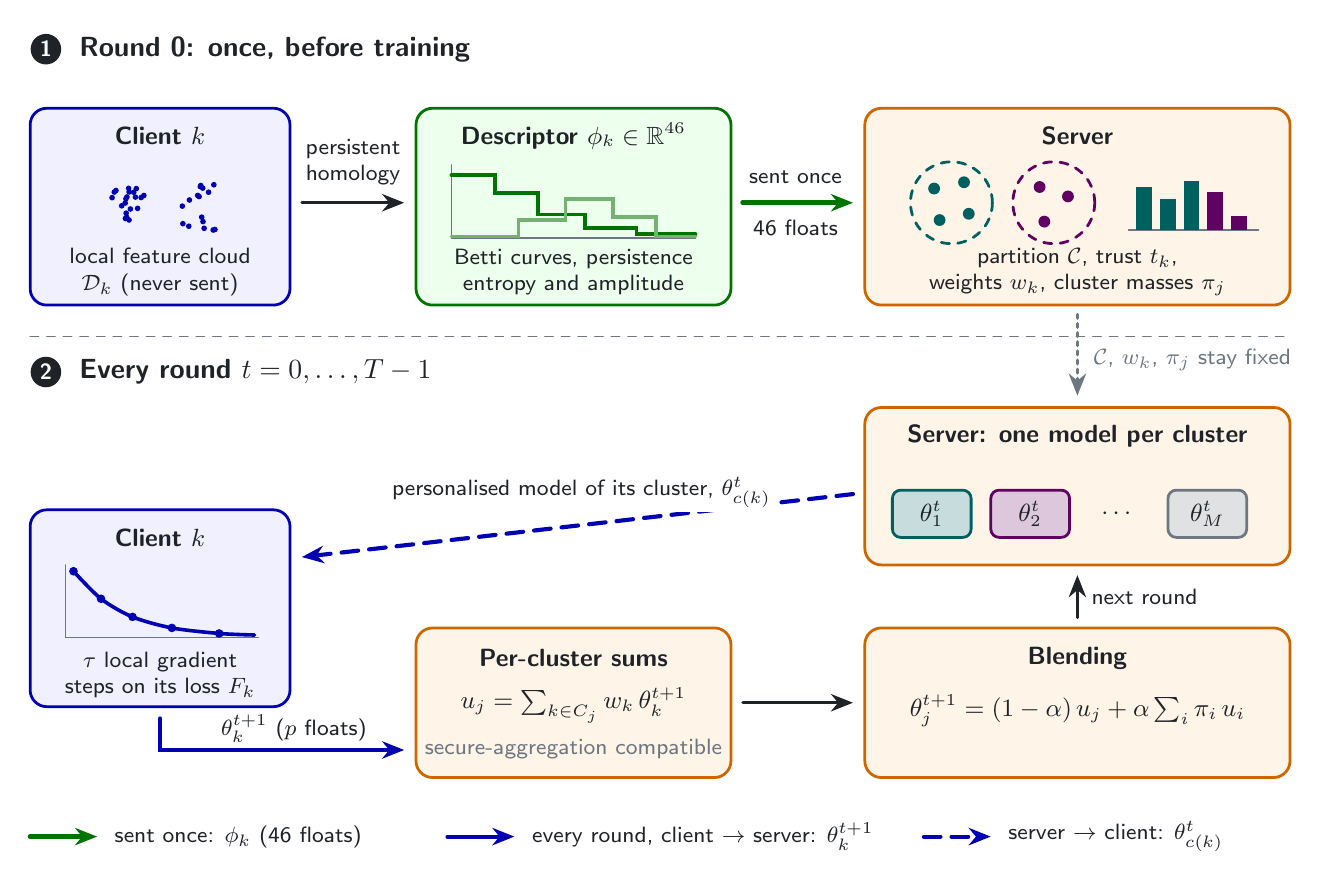
\begin{tikzpicture}[color=fg, font=\sffamily\small, line cap=round,
  >={Stealth[length=2.8mm,width=2.2mm]},
  box/.style={rounded corners=6pt, line width=1pt},
  head/.style={font=\sffamily\bfseries\small, text=fg},
  note/.style={font=\sffamily\footnotesize, text=fg, align=center},
  lab/.style={font=\sffamily\footnotesize, text=fg, fill=bg, inner sep=1.5pt, align=center},
  num/.style={circle, fill=fg, text=bg, inner sep=1.4pt, font=\sffamily\bfseries\footnotesize}]

% ============================ panel 1: round 0 ============================
\node[num] at (0.2,9.25) {1};
\node[anchor=west, font=\sffamily\bfseries\normalsize, text=fg] at (0.5,9.25) {Round 0: once, before training};

% client
\draw[box, draw=cl, fill=clfill] (0,6.0) rectangle (3.3,8.5);
\node[head] at (1.65,8.15) {Client $k$};
\pgfmathsetseed{11}
\foreach \i in {1,...,20} {\fill[cl] ({1.15+0.30*rand},{7.30+0.26*rand}) circle (0.036);}
\foreach \i in {1,...,16} {\fill[cl] ({2.15+0.22*rand},{7.25+0.32*rand}) circle (0.036);}
\node[note] at (1.65,6.42) {local feature cloud\\$\mathcal D_k$ (never sent)};

\draw[->, line width=1.1pt] (3.45,7.3) -- (4.75,7.3);
\node[note] at (4.1,7.82) {persistent\\homology};

% descriptor
\draw[box, draw=ds, fill=dsfill] (4.9,6.0) rectangle (8.9,8.5);
\node[head] at (6.9,8.15) {Descriptor $\phi_k\in\mathbb{R}^{46}$};
\draw[muted, line width=0.6pt] (5.35,6.85) -- (8.45,6.85);
\draw[muted, line width=0.6pt] (5.35,6.85) -- (5.35,7.78);
\draw[ds, line width=1.3pt] (5.35,7.65) -- (5.9,7.65) -- (5.9,7.42) -- (6.45,7.42) -- (6.45,7.15) -- (7.05,7.15)
      -- (7.05,6.98) -- (7.7,6.98) -- (7.7,6.9) -- (8.45,6.9);
\draw[ds!55!bg, line width=1.3pt] (5.35,6.87) -- (6.2,6.87) -- (6.2,7.08) -- (6.8,7.08) -- (6.8,7.35) -- (7.4,7.35)
      -- (7.4,7.12) -- (7.95,7.12) -- (7.95,6.87) -- (8.45,6.87);
\node[note] at (6.9,6.42) {Betti curves, persistence\\entropy and amplitude};

\draw[->, line width=1.8pt, draw=ds] (9.05,7.3) -- (10.45,7.3);
\node[lab] at (9.72,7.62) {sent once};
\node[lab] at (9.72,6.98) {46 floats};

% server structure
\draw[box, draw=sv, fill=svfill] (10.6,6.0) rectangle (16.0,8.5);
\node[head] at (13.3,8.15) {Server};
\draw[ca, dashed, line width=1pt] (11.7,7.3) circle (0.52);
\draw[cb, dashed, line width=1pt] (13.0,7.3) circle (0.52);
\foreach \p in {(11.48,7.48),(11.86,7.56),(11.55,7.08),(11.92,7.16)} \fill[ca] \p circle (0.075);
\foreach \p in {(12.82,7.5),(13.18,7.38),(12.88,7.06)} \fill[cb] \p circle (0.075);
\draw[muted, line width=0.6pt] (13.95,6.95) -- (15.6,6.95);
\foreach \x/\h/\c in {14.15/0.55/ca, 14.45/0.40/ca, 14.75/0.62/ca, 15.05/0.48/cb, 15.35/0.18/cb}
  \fill[\c] (\x-0.1,6.95) rectangle (\x+0.1,6.95+\h);
\node[note] at (13.3,6.42) {partition $\mathcal C$, trust $t_k$,\\weights $w_k$, cluster masses $\pi_j$};

% ============================ separator ============================
\draw[muted, dashed, line width=0.6pt] (0,5.6) -- (16,5.6);
\draw[->, muted, dotted, line width=1.3pt] (13.3,5.88) -- (13.3,4.85);
\node[lab, anchor=west, text=muted] at (13.45,5.3) {$\mathcal C$, $w_k$, $\pi_j$ stay fixed};

% ============================ panel 2: every round ============================
\node[num] at (0.2,5.15) {2};
\node[anchor=west, font=\sffamily\bfseries\normalsize, text=fg] at (0.5,5.15) {Every round $t=0,\dots,T-1$};

% server models
\draw[box, draw=sv, fill=svfill] (10.6,2.7) rectangle (16.0,4.7);
\node[head] at (13.3,4.33) {Server: one model per cluster};
\foreach \x/\c/\t in {11.45/ca/1, 12.7/cb/2, 14.95/muted/M}
  {\draw[\c, fill=\c!22!bg, rounded corners=3pt, line width=1pt] (\x-0.5,3.05) rectangle (\x+0.5,3.65);
   \node[text=fg] at (\x,3.35) {$\theta^{t}_{\t}$};}
\node[text=fg] at (13.82,3.35) {$\cdots$};

% client training
\draw[box, draw=cl, fill=clfill] (0,0.9) rectangle (3.3,3.4);
\node[head] at (1.65,3.05) {Client $k$};
\draw[muted, line width=0.6pt] (0.45,1.78) -- (2.9,1.78);
\draw[muted, line width=0.6pt] (0.45,1.78) -- (0.45,2.7);
\draw[cl, line width=1.3pt] plot[smooth] coordinates {(0.55,2.62) (0.9,2.27) (1.3,2.04) (1.8,1.9) (2.4,1.83) (2.85,1.81)};
\foreach \p in {(0.55,2.62),(0.9,2.27),(1.3,2.04),(1.8,1.9),(2.4,1.83)} \fill[cl] \p circle (0.055);
\node[note] at (1.65,1.3) {$\tau$ local gradient\\steps on its loss $F_k$};

% broadcast (dashed) and upload (solid)
\draw[->, line width=1.5pt, draw=cl, dash pattern=on 6pt off 4pt] (10.45,3.6) -- (3.45,2.8);
\node[lab] at (7.0,3.62) {personalised model of its cluster, $\theta^{t}_{c(k)}$};
\draw[->, line width=1.5pt, draw=cl] (1.65,0.75) |- (4.75,0.35);
\node[lab] at (3.35,0.62) {$\theta^{t+1}_k$ ($p$ floats)};

% aggregation and blending
\draw[box, draw=sv, fill=svfill] (4.9,0) rectangle (8.9,1.9);
\node[head] at (6.9,1.52) {Per-cluster sums};
\node[text=fg] at (6.9,0.92) {$u_j=\sum_{k\in C_j} w_k\,\theta^{t+1}_k$};
\node[note, text=muted] at (6.9,0.36) {secure-aggregation compatible};
\draw[->, line width=1.1pt] (9.05,0.95) -- (10.45,0.95);
\draw[box, draw=sv, fill=svfill] (10.6,0) rectangle (16.0,1.9);
\node[head] at (13.3,1.52) {Blending};
\node[text=fg] at (13.3,0.85) {$\theta^{t+1}_j=(1-\alpha)\,u_j+\alpha\sum_i\pi_i\,u_i$};
\draw[->, line width=1.1pt] (13.3,2.03) -- (13.3,2.57);
\node[lab, anchor=west] at (13.42,2.3) {next round};

% ============================ legend ============================
\draw[->, line width=1.8pt, draw=ds] (0,-0.75) -- (0.85,-0.75);
\node[anchor=west, font=\sffamily\footnotesize] at (0.95,-0.75) {sent once: $\phi_k$ (46 floats)};
\draw[->, line width=1.5pt, draw=cl] (5.3,-0.75) -- (6.15,-0.75);
\node[anchor=west, font=\sffamily\footnotesize] at (6.25,-0.75) {every round, client $\to$ server: $\theta^{t+1}_k$};
\draw[->, line width=1.5pt, draw=cl, dash pattern=on 6pt off 4pt] (11.35,-0.75) -- (12.2,-0.75);
\node[anchor=west, font=\sffamily\footnotesize] at (12.3,-0.75) {server $\to$ client: $\theta^{t}_{c(k)}$};
\end{tikzpicture}
\end{document}
"
%   pdftocairo -svg <name>.pdf <name>.svg   (and pdftoppm -png -r 300 -singlefile <name>.pdf <name>)
\documentclass[border=14pt]{standalone}
\usepackage{amsmath,amssymb}
\usepackage[scaled=0.92]{helvet}
\renewcommand{\familydefault}{\sfdefault}
\usepackage{tikz}
\usetikzlibrary{arrows.meta,calc}
\providecommand{\isdark}{0}
\ifnum\isdark=1
  \definecolor{bg}{HTML}{0D1117}\definecolor{fg}{HTML}{E6EDF3}\definecolor{muted}{HTML}{8B949E}
  \colorlet{cl}{blue!35!white}\colorlet{clfill}{blue!16!bg}
  \colorlet{ds}{green!65!white}\colorlet{dsfill}{green!12!bg}
  \colorlet{sv}{orange!80!white}\colorlet{svfill}{orange!13!bg}
  \colorlet{ca}{cyan!75!white}\colorlet{cb}{magenta!55!white}
\else
  \definecolor{bg}{HTML}{FFFFFF}\definecolor{fg}{HTML}{1F2328}\definecolor{muted}{HTML}{6E7781}
  \colorlet{cl}{blue!70!black}\colorlet{clfill}{blue!6}
  \colorlet{ds}{green!45!black}\colorlet{dsfill}{green!7}
  \colorlet{sv}{orange!80!black}\colorlet{svfill}{orange!9}
  \colorlet{ca}{teal!75!black}\colorlet{cb}{violet!75!black}
\fi
\pagecolor{bg}
\begin{document}
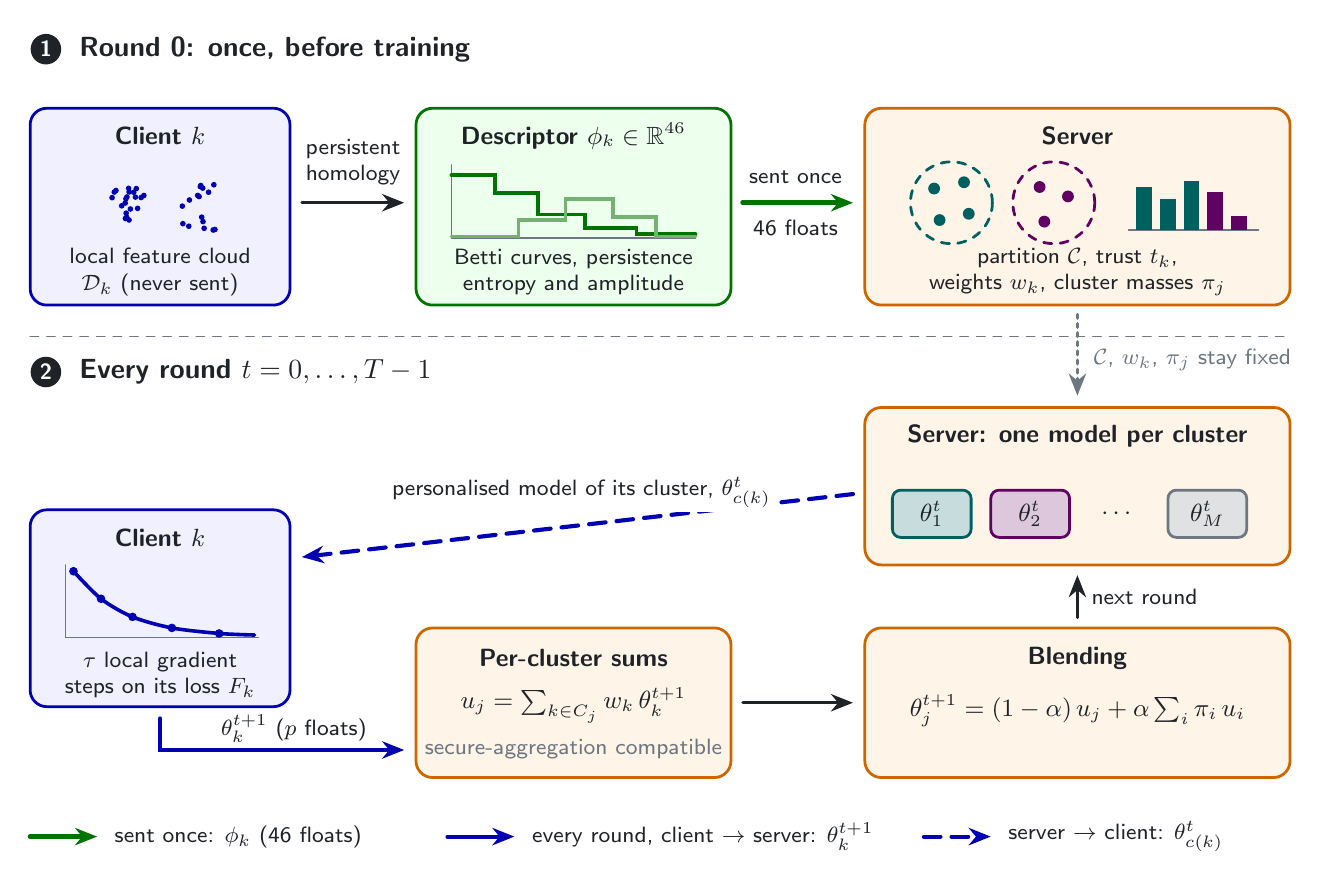
\begin{tikzpicture}[color=fg, font=\sffamily\small, line cap=round,
  >={Stealth[length=2.8mm,width=2.2mm]},
  box/.style={rounded corners=6pt, line width=1pt},
  head/.style={font=\sffamily\bfseries\small, text=fg},
  note/.style={font=\sffamily\footnotesize, text=fg, align=center},
  lab/.style={font=\sffamily\footnotesize, text=fg, fill=bg, inner sep=1.5pt, align=center},
  num/.style={circle, fill=fg, text=bg, inner sep=1.4pt, font=\sffamily\bfseries\footnotesize}]

% ============================ panel 1: round 0 ============================
\node[num] at (0.2,9.25) {1};
\node[anchor=west, font=\sffamily\bfseries\normalsize, text=fg] at (0.5,9.25) {Round 0: once, before training};

% client
\draw[box, draw=cl, fill=clfill] (0,6.0) rectangle (3.3,8.5);
\node[head] at (1.65,8.15) {Client $k$};
\pgfmathsetseed{11}
\foreach \i in {1,...,20} {\fill[cl] ({1.15+0.30*rand},{7.30+0.26*rand}) circle (0.036);}
\foreach \i in {1,...,16} {\fill[cl] ({2.15+0.22*rand},{7.25+0.32*rand}) circle (0.036);}
\node[note] at (1.65,6.42) {local feature cloud\\$\mathcal D_k$ (never sent)};

\draw[->, line width=1.1pt] (3.45,7.3) -- (4.75,7.3);
\node[note] at (4.1,7.82) {persistent\\homology};

% descriptor
\draw[box, draw=ds, fill=dsfill] (4.9,6.0) rectangle (8.9,8.5);
\node[head] at (6.9,8.15) {Descriptor $\phi_k\in\mathbb{R}^{46}$};
\draw[muted, line width=0.6pt] (5.35,6.85) -- (8.45,6.85);
\draw[muted, line width=0.6pt] (5.35,6.85) -- (5.35,7.78);
\draw[ds, line width=1.3pt] (5.35,7.65) -- (5.9,7.65) -- (5.9,7.42) -- (6.45,7.42) -- (6.45,7.15) -- (7.05,7.15)
      -- (7.05,6.98) -- (7.7,6.98) -- (7.7,6.9) -- (8.45,6.9);
\draw[ds!55!bg, line width=1.3pt] (5.35,6.87) -- (6.2,6.87) -- (6.2,7.08) -- (6.8,7.08) -- (6.8,7.35) -- (7.4,7.35)
      -- (7.4,7.12) -- (7.95,7.12) -- (7.95,6.87) -- (8.45,6.87);
\node[note] at (6.9,6.42) {Betti curves, persistence\\entropy and amplitude};

\draw[->, line width=1.8pt, draw=ds] (9.05,7.3) -- (10.45,7.3);
\node[lab] at (9.72,7.62) {sent once};
\node[lab] at (9.72,6.98) {46 floats};

% server structure
\draw[box, draw=sv, fill=svfill] (10.6,6.0) rectangle (16.0,8.5);
\node[head] at (13.3,8.15) {Server};
\draw[ca, dashed, line width=1pt] (11.7,7.3) circle (0.52);
\draw[cb, dashed, line width=1pt] (13.0,7.3) circle (0.52);
\foreach \p in {(11.48,7.48),(11.86,7.56),(11.55,7.08),(11.92,7.16)} \fill[ca] \p circle (0.075);
\foreach \p in {(12.82,7.5),(13.18,7.38),(12.88,7.06)} \fill[cb] \p circle (0.075);
\draw[muted, line width=0.6pt] (13.95,6.95) -- (15.6,6.95);
\foreach \x/\h/\c in {14.15/0.55/ca, 14.45/0.40/ca, 14.75/0.62/ca, 15.05/0.48/cb, 15.35/0.18/cb}
  \fill[\c] (\x-0.1,6.95) rectangle (\x+0.1,6.95+\h);
\node[note] at (13.3,6.42) {partition $\mathcal C$, trust $t_k$,\\weights $w_k$, cluster masses $\pi_j$};

% ============================ separator ============================
\draw[muted, dashed, line width=0.6pt] (0,5.6) -- (16,5.6);
\draw[->, muted, dotted, line width=1.3pt] (13.3,5.88) -- (13.3,4.85);
\node[lab, anchor=west, text=muted] at (13.45,5.3) {$\mathcal C$, $w_k$, $\pi_j$ stay fixed};

% ============================ panel 2: every round ============================
\node[num] at (0.2,5.15) {2};
\node[anchor=west, font=\sffamily\bfseries\normalsize, text=fg] at (0.5,5.15) {Every round $t=0,\dots,T-1$};

% server models
\draw[box, draw=sv, fill=svfill] (10.6,2.7) rectangle (16.0,4.7);
\node[head] at (13.3,4.33) {Server: one model per cluster};
\foreach \x/\c/\t in {11.45/ca/1, 12.7/cb/2, 14.95/muted/M}
  {\draw[\c, fill=\c!22!bg, rounded corners=3pt, line width=1pt] (\x-0.5,3.05) rectangle (\x+0.5,3.65);
   \node[text=fg] at (\x,3.35) {$\theta^{t}_{\t}$};}
\node[text=fg] at (13.82,3.35) {$\cdots$};

% client training
\draw[box, draw=cl, fill=clfill] (0,0.9) rectangle (3.3,3.4);
\node[head] at (1.65,3.05) {Client $k$};
\draw[muted, line width=0.6pt] (0.45,1.78) -- (2.9,1.78);
\draw[muted, line width=0.6pt] (0.45,1.78) -- (0.45,2.7);
\draw[cl, line width=1.3pt] plot[smooth] coordinates {(0.55,2.62) (0.9,2.27) (1.3,2.04) (1.8,1.9) (2.4,1.83) (2.85,1.81)};
\foreach \p in {(0.55,2.62),(0.9,2.27),(1.3,2.04),(1.8,1.9),(2.4,1.83)} \fill[cl] \p circle (0.055);
\node[note] at (1.65,1.3) {$\tau$ local gradient\\steps on its loss $F_k$};

% broadcast (dashed) and upload (solid)
\draw[->, line width=1.5pt, draw=cl, dash pattern=on 6pt off 4pt] (10.45,3.6) -- (3.45,2.8);
\node[lab] at (7.0,3.62) {personalised model of its cluster, $\theta^{t}_{c(k)}$};
\draw[->, line width=1.5pt, draw=cl] (1.65,0.75) |- (4.75,0.35);
\node[lab] at (3.35,0.62) {$\theta^{t+1}_k$ ($p$ floats)};

% aggregation and blending
\draw[box, draw=sv, fill=svfill] (4.9,0) rectangle (8.9,1.9);
\node[head] at (6.9,1.52) {Per-cluster sums};
\node[text=fg] at (6.9,0.92) {$u_j=\sum_{k\in C_j} w_k\,\theta^{t+1}_k$};
\node[note, text=muted] at (6.9,0.36) {secure-aggregation compatible};
\draw[->, line width=1.1pt] (9.05,0.95) -- (10.45,0.95);
\draw[box, draw=sv, fill=svfill] (10.6,0) rectangle (16.0,1.9);
\node[head] at (13.3,1.52) {Blending};
\node[text=fg] at (13.3,0.85) {$\theta^{t+1}_j=(1-\alpha)\,u_j+\alpha\sum_i\pi_i\,u_i$};
\draw[->, line width=1.1pt] (13.3,2.03) -- (13.3,2.57);
\node[lab, anchor=west] at (13.42,2.3) {next round};

% ============================ legend ============================
\draw[->, line width=1.8pt, draw=ds] (0,-0.75) -- (0.85,-0.75);
\node[anchor=west, font=\sffamily\footnotesize] at (0.95,-0.75) {sent once: $\phi_k$ (46 floats)};
\draw[->, line width=1.5pt, draw=cl] (5.3,-0.75) -- (6.15,-0.75);
\node[anchor=west, font=\sffamily\footnotesize] at (6.25,-0.75) {every round, client $\to$ server: $\theta^{t+1}_k$};
\draw[->, line width=1.5pt, draw=cl, dash pattern=on 6pt off 4pt] (11.35,-0.75) -- (12.2,-0.75);
\node[anchor=west, font=\sffamily\footnotesize] at (12.3,-0.75) {server $\to$ client: $\theta^{t}_{c(k)}$};
\end{tikzpicture}
\end{document}
"
%   pdftocairo -svg <name>.pdf <name>.svg   (and pdftoppm -png -r 300 -singlefile <name>.pdf <name>)
\documentclass[border=14pt]{standalone}
\usepackage{amsmath,amssymb}
\usepackage[scaled=0.92]{helvet}
\renewcommand{\familydefault}{\sfdefault}
\usepackage{tikz}
\usetikzlibrary{arrows.meta,calc}
\providecommand{\isdark}{0}
\ifnum\isdark=1
  \definecolor{bg}{HTML}{0D1117}\definecolor{fg}{HTML}{E6EDF3}\definecolor{muted}{HTML}{8B949E}
  \colorlet{cl}{blue!35!white}\colorlet{clfill}{blue!16!bg}
  \colorlet{ds}{green!65!white}\colorlet{dsfill}{green!12!bg}
  \colorlet{sv}{orange!80!white}\colorlet{svfill}{orange!13!bg}
  \colorlet{ca}{cyan!75!white}\colorlet{cb}{magenta!55!white}
\else
  \definecolor{bg}{HTML}{FFFFFF}\definecolor{fg}{HTML}{1F2328}\definecolor{muted}{HTML}{6E7781}
  \colorlet{cl}{blue!70!black}\colorlet{clfill}{blue!6}
  \colorlet{ds}{green!45!black}\colorlet{dsfill}{green!7}
  \colorlet{sv}{orange!80!black}\colorlet{svfill}{orange!9}
  \colorlet{ca}{teal!75!black}\colorlet{cb}{violet!75!black}
\fi
\pagecolor{bg}
\begin{document}
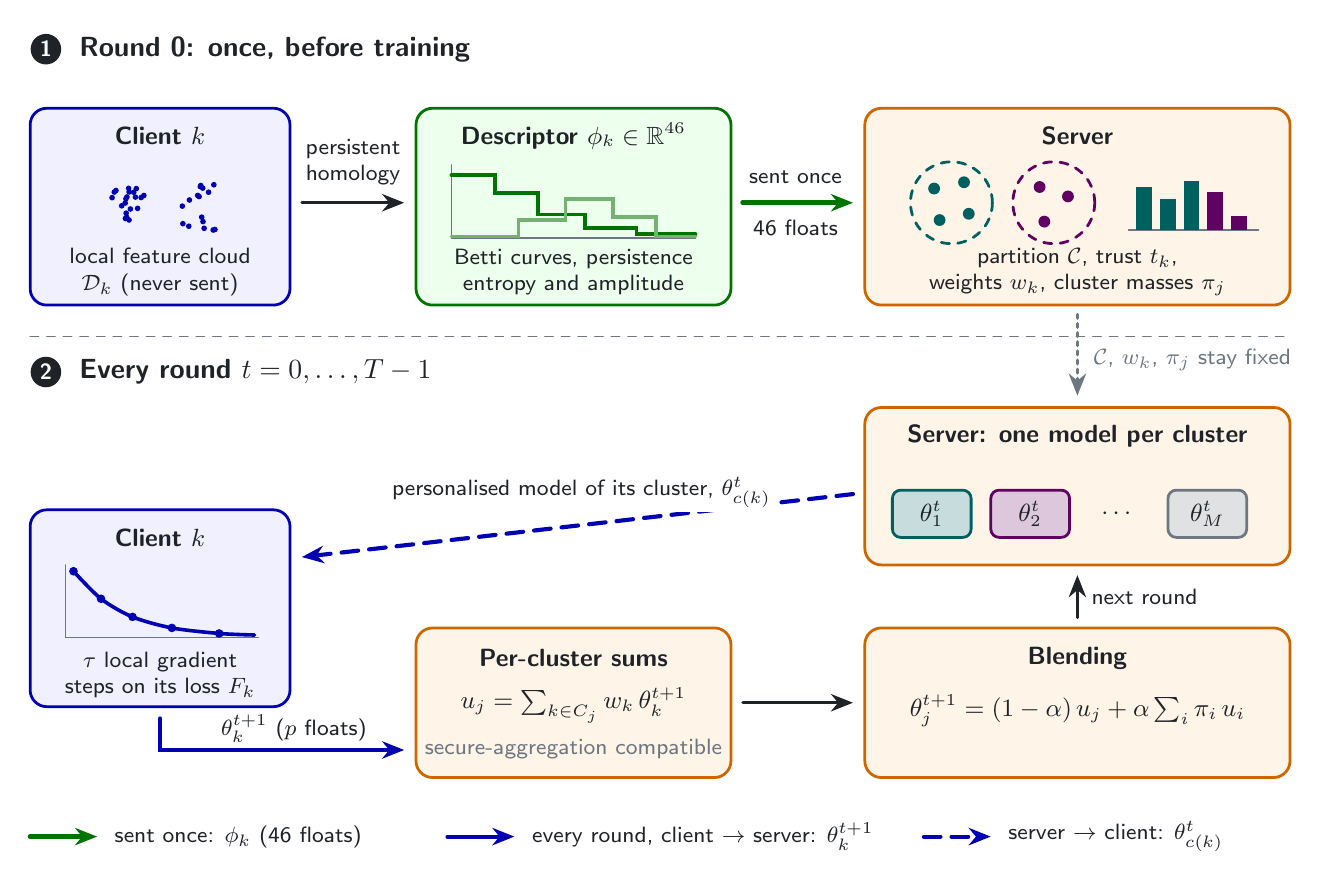
\begin{tikzpicture}[color=fg, font=\sffamily\small, line cap=round,
  >={Stealth[length=2.8mm,width=2.2mm]},
  box/.style={rounded corners=6pt, line width=1pt},
  head/.style={font=\sffamily\bfseries\small, text=fg},
  note/.style={font=\sffamily\footnotesize, text=fg, align=center},
  lab/.style={font=\sffamily\footnotesize, text=fg, fill=bg, inner sep=1.5pt, align=center},
  num/.style={circle, fill=fg, text=bg, inner sep=1.4pt, font=\sffamily\bfseries\footnotesize}]

% ============================ panel 1: round 0 ============================
\node[num] at (0.2,9.25) {1};
\node[anchor=west, font=\sffamily\bfseries\normalsize, text=fg] at (0.5,9.25) {Round 0: once, before training};

% client
\draw[box, draw=cl, fill=clfill] (0,6.0) rectangle (3.3,8.5);
\node[head] at (1.65,8.15) {Client $k$};
\pgfmathsetseed{11}
\foreach \i in {1,...,20} {\fill[cl] ({1.15+0.30*rand},{7.30+0.26*rand}) circle (0.036);}
\foreach \i in {1,...,16} {\fill[cl] ({2.15+0.22*rand},{7.25+0.32*rand}) circle (0.036);}
\node[note] at (1.65,6.42) {local feature cloud\\$\mathcal D_k$ (never sent)};

\draw[->, line width=1.1pt] (3.45,7.3) -- (4.75,7.3);
\node[note] at (4.1,7.82) {persistent\\homology};

% descriptor
\draw[box, draw=ds, fill=dsfill] (4.9,6.0) rectangle (8.9,8.5);
\node[head] at (6.9,8.15) {Descriptor $\phi_k\in\mathbb{R}^{46}$};
\draw[muted, line width=0.6pt] (5.35,6.85) -- (8.45,6.85);
\draw[muted, line width=0.6pt] (5.35,6.85) -- (5.35,7.78);
\draw[ds, line width=1.3pt] (5.35,7.65) -- (5.9,7.65) -- (5.9,7.42) -- (6.45,7.42) -- (6.45,7.15) -- (7.05,7.15)
      -- (7.05,6.98) -- (7.7,6.98) -- (7.7,6.9) -- (8.45,6.9);
\draw[ds!55!bg, line width=1.3pt] (5.35,6.87) -- (6.2,6.87) -- (6.2,7.08) -- (6.8,7.08) -- (6.8,7.35) -- (7.4,7.35)
      -- (7.4,7.12) -- (7.95,7.12) -- (7.95,6.87) -- (8.45,6.87);
\node[note] at (6.9,6.42) {Betti curves, persistence\\entropy and amplitude};

\draw[->, line width=1.8pt, draw=ds] (9.05,7.3) -- (10.45,7.3);
\node[lab] at (9.72,7.62) {sent once};
\node[lab] at (9.72,6.98) {46 floats};

% server structure
\draw[box, draw=sv, fill=svfill] (10.6,6.0) rectangle (16.0,8.5);
\node[head] at (13.3,8.15) {Server};
\draw[ca, dashed, line width=1pt] (11.7,7.3) circle (0.52);
\draw[cb, dashed, line width=1pt] (13.0,7.3) circle (0.52);
\foreach \p in {(11.48,7.48),(11.86,7.56),(11.55,7.08),(11.92,7.16)} \fill[ca] \p circle (0.075);
\foreach \p in {(12.82,7.5),(13.18,7.38),(12.88,7.06)} \fill[cb] \p circle (0.075);
\draw[muted, line width=0.6pt] (13.95,6.95) -- (15.6,6.95);
\foreach \x/\h/\c in {14.15/0.55/ca, 14.45/0.40/ca, 14.75/0.62/ca, 15.05/0.48/cb, 15.35/0.18/cb}
  \fill[\c] (\x-0.1,6.95) rectangle (\x+0.1,6.95+\h);
\node[note] at (13.3,6.42) {partition $\mathcal C$, trust $t_k$,\\weights $w_k$, cluster masses $\pi_j$};

% ============================ separator ============================
\draw[muted, dashed, line width=0.6pt] (0,5.6) -- (16,5.6);
\draw[->, muted, dotted, line width=1.3pt] (13.3,5.88) -- (13.3,4.85);
\node[lab, anchor=west, text=muted] at (13.45,5.3) {$\mathcal C$, $w_k$, $\pi_j$ stay fixed};

% ============================ panel 2: every round ============================
\node[num] at (0.2,5.15) {2};
\node[anchor=west, font=\sffamily\bfseries\normalsize, text=fg] at (0.5,5.15) {Every round $t=0,\dots,T-1$};

% server models
\draw[box, draw=sv, fill=svfill] (10.6,2.7) rectangle (16.0,4.7);
\node[head] at (13.3,4.33) {Server: one model per cluster};
\foreach \x/\c/\t in {11.45/ca/1, 12.7/cb/2, 14.95/muted/M}
  {\draw[\c, fill=\c!22!bg, rounded corners=3pt, line width=1pt] (\x-0.5,3.05) rectangle (\x+0.5,3.65);
   \node[text=fg] at (\x,3.35) {$\theta^{t}_{\t}$};}
\node[text=fg] at (13.82,3.35) {$\cdots$};

% client training
\draw[box, draw=cl, fill=clfill] (0,0.9) rectangle (3.3,3.4);
\node[head] at (1.65,3.05) {Client $k$};
\draw[muted, line width=0.6pt] (0.45,1.78) -- (2.9,1.78);
\draw[muted, line width=0.6pt] (0.45,1.78) -- (0.45,2.7);
\draw[cl, line width=1.3pt] plot[smooth] coordinates {(0.55,2.62) (0.9,2.27) (1.3,2.04) (1.8,1.9) (2.4,1.83) (2.85,1.81)};
\foreach \p in {(0.55,2.62),(0.9,2.27),(1.3,2.04),(1.8,1.9),(2.4,1.83)} \fill[cl] \p circle (0.055);
\node[note] at (1.65,1.3) {$\tau$ local gradient\\steps on its loss $F_k$};

% broadcast (dashed) and upload (solid)
\draw[->, line width=1.5pt, draw=cl, dash pattern=on 6pt off 4pt] (10.45,3.6) -- (3.45,2.8);
\node[lab] at (7.0,3.62) {personalised model of its cluster, $\theta^{t}_{c(k)}$};
\draw[->, line width=1.5pt, draw=cl] (1.65,0.75) |- (4.75,0.35);
\node[lab] at (3.35,0.62) {$\theta^{t+1}_k$ ($p$ floats)};

% aggregation and blending
\draw[box, draw=sv, fill=svfill] (4.9,0) rectangle (8.9,1.9);
\node[head] at (6.9,1.52) {Per-cluster sums};
\node[text=fg] at (6.9,0.92) {$u_j=\sum_{k\in C_j} w_k\,\theta^{t+1}_k$};
\node[note, text=muted] at (6.9,0.36) {secure-aggregation compatible};
\draw[->, line width=1.1pt] (9.05,0.95) -- (10.45,0.95);
\draw[box, draw=sv, fill=svfill] (10.6,0) rectangle (16.0,1.9);
\node[head] at (13.3,1.52) {Blending};
\node[text=fg] at (13.3,0.85) {$\theta^{t+1}_j=(1-\alpha)\,u_j+\alpha\sum_i\pi_i\,u_i$};
\draw[->, line width=1.1pt] (13.3,2.03) -- (13.3,2.57);
\node[lab, anchor=west] at (13.42,2.3) {next round};

% ============================ legend ============================
\draw[->, line width=1.8pt, draw=ds] (0,-0.75) -- (0.85,-0.75);
\node[anchor=west, font=\sffamily\footnotesize] at (0.95,-0.75) {sent once: $\phi_k$ (46 floats)};
\draw[->, line width=1.5pt, draw=cl] (5.3,-0.75) -- (6.15,-0.75);
\node[anchor=west, font=\sffamily\footnotesize] at (6.25,-0.75) {every round, client $\to$ server: $\theta^{t+1}_k$};
\draw[->, line width=1.5pt, draw=cl, dash pattern=on 6pt off 4pt] (11.35,-0.75) -- (12.2,-0.75);
\node[anchor=west, font=\sffamily\footnotesize] at (12.3,-0.75) {server $\to$ client: $\theta^{t}_{c(k)}$};
\end{tikzpicture}
\end{document}
"
%   pdflatex -jobname=ptopofl_protocol_dark  "\def\isdark{1}% pTopoFL protocol figure for the README.  Build:
%   pdflatex -jobname=ptopofl_protocol_light "\def\isdark{0}% pTopoFL protocol figure for the README.  Build:
%   pdflatex -jobname=ptopofl_protocol_light "\def\isdark{0}% pTopoFL protocol figure for the README.  Build:
%   pdflatex -jobname=ptopofl_protocol_light "\def\isdark{0}\input{ptopofl_protocol}"
%   pdflatex -jobname=ptopofl_protocol_dark  "\def\isdark{1}\input{ptopofl_protocol}"
%   pdftocairo -svg <name>.pdf <name>.svg   (and pdftoppm -png -r 300 -singlefile <name>.pdf <name>)
\documentclass[border=14pt]{standalone}
\usepackage{amsmath,amssymb}
\usepackage[scaled=0.92]{helvet}
\renewcommand{\familydefault}{\sfdefault}
\usepackage{tikz}
\usetikzlibrary{arrows.meta,calc}
\providecommand{\isdark}{0}
\ifnum\isdark=1
  \definecolor{bg}{HTML}{0D1117}\definecolor{fg}{HTML}{E6EDF3}\definecolor{muted}{HTML}{8B949E}
  \colorlet{cl}{blue!35!white}\colorlet{clfill}{blue!16!bg}
  \colorlet{ds}{green!65!white}\colorlet{dsfill}{green!12!bg}
  \colorlet{sv}{orange!80!white}\colorlet{svfill}{orange!13!bg}
  \colorlet{ca}{cyan!75!white}\colorlet{cb}{magenta!55!white}
\else
  \definecolor{bg}{HTML}{FFFFFF}\definecolor{fg}{HTML}{1F2328}\definecolor{muted}{HTML}{6E7781}
  \colorlet{cl}{blue!70!black}\colorlet{clfill}{blue!6}
  \colorlet{ds}{green!45!black}\colorlet{dsfill}{green!7}
  \colorlet{sv}{orange!80!black}\colorlet{svfill}{orange!9}
  \colorlet{ca}{teal!75!black}\colorlet{cb}{violet!75!black}
\fi
\pagecolor{bg}
\begin{document}
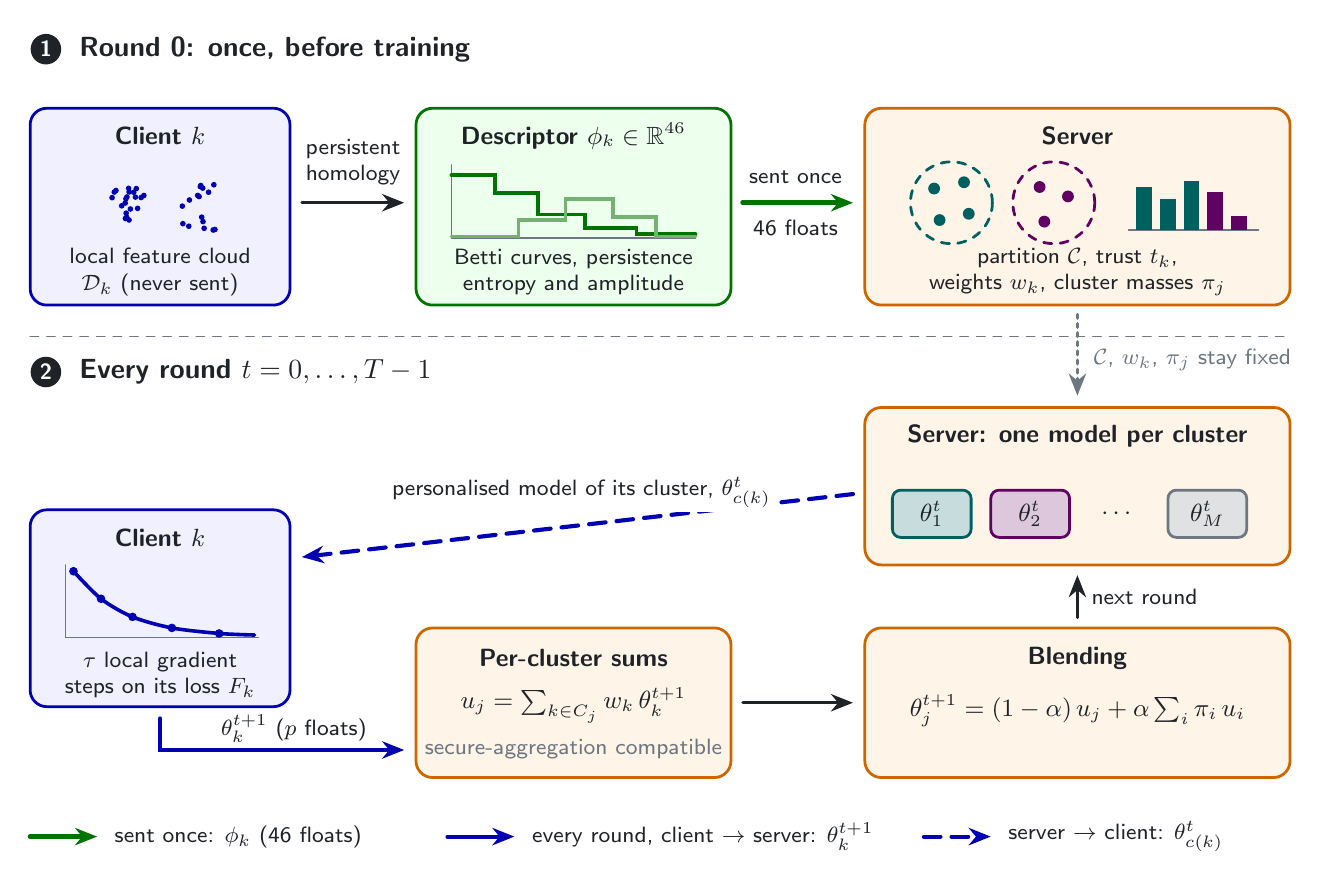
\begin{tikzpicture}[color=fg, font=\sffamily\small, line cap=round,
  >={Stealth[length=2.8mm,width=2.2mm]},
  box/.style={rounded corners=6pt, line width=1pt},
  head/.style={font=\sffamily\bfseries\small, text=fg},
  note/.style={font=\sffamily\footnotesize, text=fg, align=center},
  lab/.style={font=\sffamily\footnotesize, text=fg, fill=bg, inner sep=1.5pt, align=center},
  num/.style={circle, fill=fg, text=bg, inner sep=1.4pt, font=\sffamily\bfseries\footnotesize}]

% ============================ panel 1: round 0 ============================
\node[num] at (0.2,9.25) {1};
\node[anchor=west, font=\sffamily\bfseries\normalsize, text=fg] at (0.5,9.25) {Round 0: once, before training};

% client
\draw[box, draw=cl, fill=clfill] (0,6.0) rectangle (3.3,8.5);
\node[head] at (1.65,8.15) {Client $k$};
\pgfmathsetseed{11}
\foreach \i in {1,...,20} {\fill[cl] ({1.15+0.30*rand},{7.30+0.26*rand}) circle (0.036);}
\foreach \i in {1,...,16} {\fill[cl] ({2.15+0.22*rand},{7.25+0.32*rand}) circle (0.036);}
\node[note] at (1.65,6.42) {local feature cloud\\$\mathcal D_k$ (never sent)};

\draw[->, line width=1.1pt] (3.45,7.3) -- (4.75,7.3);
\node[note] at (4.1,7.82) {persistent\\homology};

% descriptor
\draw[box, draw=ds, fill=dsfill] (4.9,6.0) rectangle (8.9,8.5);
\node[head] at (6.9,8.15) {Descriptor $\phi_k\in\mathbb{R}^{46}$};
\draw[muted, line width=0.6pt] (5.35,6.85) -- (8.45,6.85);
\draw[muted, line width=0.6pt] (5.35,6.85) -- (5.35,7.78);
\draw[ds, line width=1.3pt] (5.35,7.65) -- (5.9,7.65) -- (5.9,7.42) -- (6.45,7.42) -- (6.45,7.15) -- (7.05,7.15)
      -- (7.05,6.98) -- (7.7,6.98) -- (7.7,6.9) -- (8.45,6.9);
\draw[ds!55!bg, line width=1.3pt] (5.35,6.87) -- (6.2,6.87) -- (6.2,7.08) -- (6.8,7.08) -- (6.8,7.35) -- (7.4,7.35)
      -- (7.4,7.12) -- (7.95,7.12) -- (7.95,6.87) -- (8.45,6.87);
\node[note] at (6.9,6.42) {Betti curves, persistence\\entropy and amplitude};

\draw[->, line width=1.8pt, draw=ds] (9.05,7.3) -- (10.45,7.3);
\node[lab] at (9.72,7.62) {sent once};
\node[lab] at (9.72,6.98) {46 floats};

% server structure
\draw[box, draw=sv, fill=svfill] (10.6,6.0) rectangle (16.0,8.5);
\node[head] at (13.3,8.15) {Server};
\draw[ca, dashed, line width=1pt] (11.7,7.3) circle (0.52);
\draw[cb, dashed, line width=1pt] (13.0,7.3) circle (0.52);
\foreach \p in {(11.48,7.48),(11.86,7.56),(11.55,7.08),(11.92,7.16)} \fill[ca] \p circle (0.075);
\foreach \p in {(12.82,7.5),(13.18,7.38),(12.88,7.06)} \fill[cb] \p circle (0.075);
\draw[muted, line width=0.6pt] (13.95,6.95) -- (15.6,6.95);
\foreach \x/\h/\c in {14.15/0.55/ca, 14.45/0.40/ca, 14.75/0.62/ca, 15.05/0.48/cb, 15.35/0.18/cb}
  \fill[\c] (\x-0.1,6.95) rectangle (\x+0.1,6.95+\h);
\node[note] at (13.3,6.42) {partition $\mathcal C$, trust $t_k$,\\weights $w_k$, cluster masses $\pi_j$};

% ============================ separator ============================
\draw[muted, dashed, line width=0.6pt] (0,5.6) -- (16,5.6);
\draw[->, muted, dotted, line width=1.3pt] (13.3,5.88) -- (13.3,4.85);
\node[lab, anchor=west, text=muted] at (13.45,5.3) {$\mathcal C$, $w_k$, $\pi_j$ stay fixed};

% ============================ panel 2: every round ============================
\node[num] at (0.2,5.15) {2};
\node[anchor=west, font=\sffamily\bfseries\normalsize, text=fg] at (0.5,5.15) {Every round $t=0,\dots,T-1$};

% server models
\draw[box, draw=sv, fill=svfill] (10.6,2.7) rectangle (16.0,4.7);
\node[head] at (13.3,4.33) {Server: one model per cluster};
\foreach \x/\c/\t in {11.45/ca/1, 12.7/cb/2, 14.95/muted/M}
  {\draw[\c, fill=\c!22!bg, rounded corners=3pt, line width=1pt] (\x-0.5,3.05) rectangle (\x+0.5,3.65);
   \node[text=fg] at (\x,3.35) {$\theta^{t}_{\t}$};}
\node[text=fg] at (13.82,3.35) {$\cdots$};

% client training
\draw[box, draw=cl, fill=clfill] (0,0.9) rectangle (3.3,3.4);
\node[head] at (1.65,3.05) {Client $k$};
\draw[muted, line width=0.6pt] (0.45,1.78) -- (2.9,1.78);
\draw[muted, line width=0.6pt] (0.45,1.78) -- (0.45,2.7);
\draw[cl, line width=1.3pt] plot[smooth] coordinates {(0.55,2.62) (0.9,2.27) (1.3,2.04) (1.8,1.9) (2.4,1.83) (2.85,1.81)};
\foreach \p in {(0.55,2.62),(0.9,2.27),(1.3,2.04),(1.8,1.9),(2.4,1.83)} \fill[cl] \p circle (0.055);
\node[note] at (1.65,1.3) {$\tau$ local gradient\\steps on its loss $F_k$};

% broadcast (dashed) and upload (solid)
\draw[->, line width=1.5pt, draw=cl, dash pattern=on 6pt off 4pt] (10.45,3.6) -- (3.45,2.8);
\node[lab] at (7.0,3.62) {personalised model of its cluster, $\theta^{t}_{c(k)}$};
\draw[->, line width=1.5pt, draw=cl] (1.65,0.75) |- (4.75,0.35);
\node[lab] at (3.35,0.62) {$\theta^{t+1}_k$ ($p$ floats)};

% aggregation and blending
\draw[box, draw=sv, fill=svfill] (4.9,0) rectangle (8.9,1.9);
\node[head] at (6.9,1.52) {Per-cluster sums};
\node[text=fg] at (6.9,0.92) {$u_j=\sum_{k\in C_j} w_k\,\theta^{t+1}_k$};
\node[note, text=muted] at (6.9,0.36) {secure-aggregation compatible};
\draw[->, line width=1.1pt] (9.05,0.95) -- (10.45,0.95);
\draw[box, draw=sv, fill=svfill] (10.6,0) rectangle (16.0,1.9);
\node[head] at (13.3,1.52) {Blending};
\node[text=fg] at (13.3,0.85) {$\theta^{t+1}_j=(1-\alpha)\,u_j+\alpha\sum_i\pi_i\,u_i$};
\draw[->, line width=1.1pt] (13.3,2.03) -- (13.3,2.57);
\node[lab, anchor=west] at (13.42,2.3) {next round};

% ============================ legend ============================
\draw[->, line width=1.8pt, draw=ds] (0,-0.75) -- (0.85,-0.75);
\node[anchor=west, font=\sffamily\footnotesize] at (0.95,-0.75) {sent once: $\phi_k$ (46 floats)};
\draw[->, line width=1.5pt, draw=cl] (5.3,-0.75) -- (6.15,-0.75);
\node[anchor=west, font=\sffamily\footnotesize] at (6.25,-0.75) {every round, client $\to$ server: $\theta^{t+1}_k$};
\draw[->, line width=1.5pt, draw=cl, dash pattern=on 6pt off 4pt] (11.35,-0.75) -- (12.2,-0.75);
\node[anchor=west, font=\sffamily\footnotesize] at (12.3,-0.75) {server $\to$ client: $\theta^{t}_{c(k)}$};
\end{tikzpicture}
\end{document}
"
%   pdflatex -jobname=ptopofl_protocol_dark  "\def\isdark{1}% pTopoFL protocol figure for the README.  Build:
%   pdflatex -jobname=ptopofl_protocol_light "\def\isdark{0}\input{ptopofl_protocol}"
%   pdflatex -jobname=ptopofl_protocol_dark  "\def\isdark{1}\input{ptopofl_protocol}"
%   pdftocairo -svg <name>.pdf <name>.svg   (and pdftoppm -png -r 300 -singlefile <name>.pdf <name>)
\documentclass[border=14pt]{standalone}
\usepackage{amsmath,amssymb}
\usepackage[scaled=0.92]{helvet}
\renewcommand{\familydefault}{\sfdefault}
\usepackage{tikz}
\usetikzlibrary{arrows.meta,calc}
\providecommand{\isdark}{0}
\ifnum\isdark=1
  \definecolor{bg}{HTML}{0D1117}\definecolor{fg}{HTML}{E6EDF3}\definecolor{muted}{HTML}{8B949E}
  \colorlet{cl}{blue!35!white}\colorlet{clfill}{blue!16!bg}
  \colorlet{ds}{green!65!white}\colorlet{dsfill}{green!12!bg}
  \colorlet{sv}{orange!80!white}\colorlet{svfill}{orange!13!bg}
  \colorlet{ca}{cyan!75!white}\colorlet{cb}{magenta!55!white}
\else
  \definecolor{bg}{HTML}{FFFFFF}\definecolor{fg}{HTML}{1F2328}\definecolor{muted}{HTML}{6E7781}
  \colorlet{cl}{blue!70!black}\colorlet{clfill}{blue!6}
  \colorlet{ds}{green!45!black}\colorlet{dsfill}{green!7}
  \colorlet{sv}{orange!80!black}\colorlet{svfill}{orange!9}
  \colorlet{ca}{teal!75!black}\colorlet{cb}{violet!75!black}
\fi
\pagecolor{bg}
\begin{document}
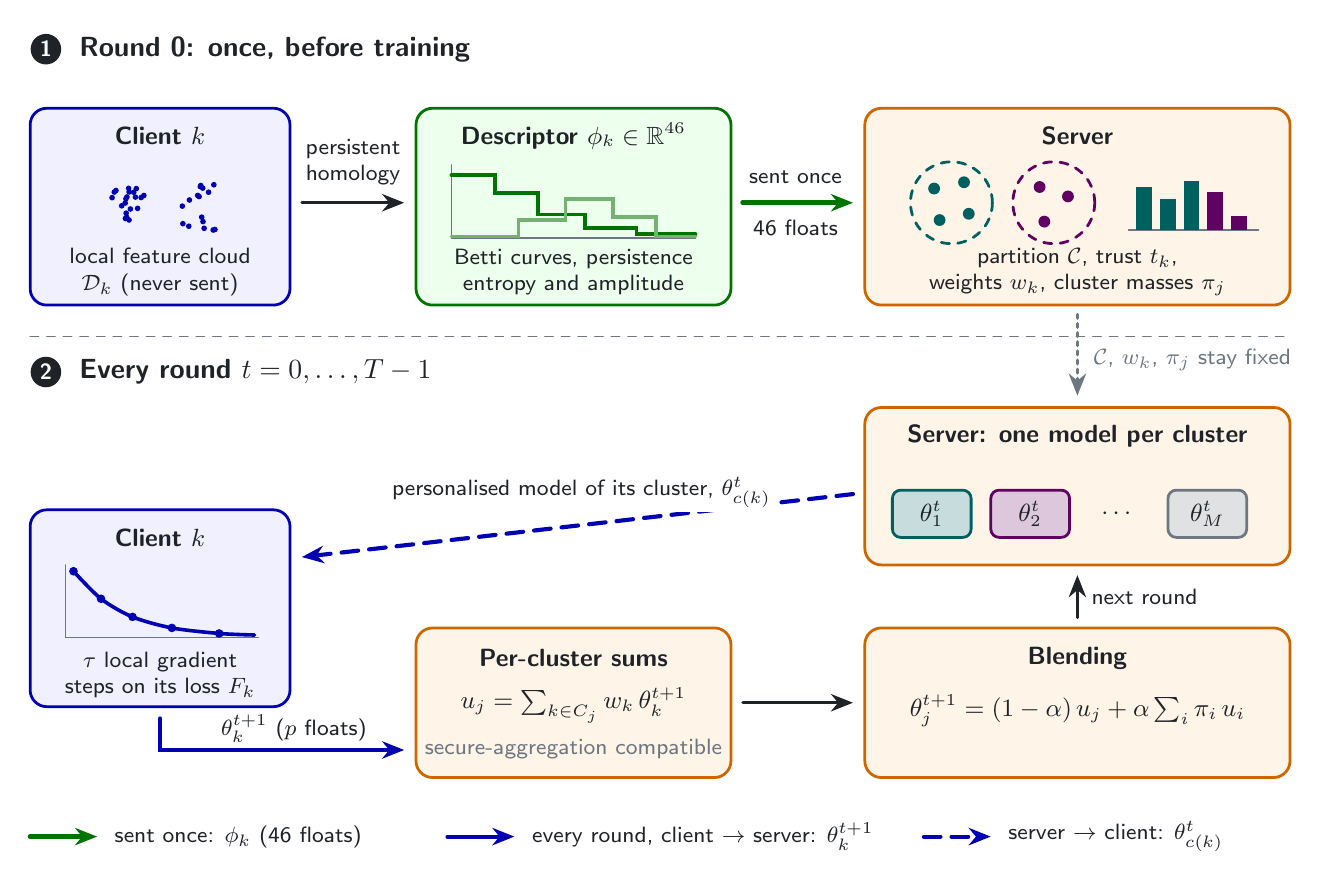
\begin{tikzpicture}[color=fg, font=\sffamily\small, line cap=round,
  >={Stealth[length=2.8mm,width=2.2mm]},
  box/.style={rounded corners=6pt, line width=1pt},
  head/.style={font=\sffamily\bfseries\small, text=fg},
  note/.style={font=\sffamily\footnotesize, text=fg, align=center},
  lab/.style={font=\sffamily\footnotesize, text=fg, fill=bg, inner sep=1.5pt, align=center},
  num/.style={circle, fill=fg, text=bg, inner sep=1.4pt, font=\sffamily\bfseries\footnotesize}]

% ============================ panel 1: round 0 ============================
\node[num] at (0.2,9.25) {1};
\node[anchor=west, font=\sffamily\bfseries\normalsize, text=fg] at (0.5,9.25) {Round 0: once, before training};

% client
\draw[box, draw=cl, fill=clfill] (0,6.0) rectangle (3.3,8.5);
\node[head] at (1.65,8.15) {Client $k$};
\pgfmathsetseed{11}
\foreach \i in {1,...,20} {\fill[cl] ({1.15+0.30*rand},{7.30+0.26*rand}) circle (0.036);}
\foreach \i in {1,...,16} {\fill[cl] ({2.15+0.22*rand},{7.25+0.32*rand}) circle (0.036);}
\node[note] at (1.65,6.42) {local feature cloud\\$\mathcal D_k$ (never sent)};

\draw[->, line width=1.1pt] (3.45,7.3) -- (4.75,7.3);
\node[note] at (4.1,7.82) {persistent\\homology};

% descriptor
\draw[box, draw=ds, fill=dsfill] (4.9,6.0) rectangle (8.9,8.5);
\node[head] at (6.9,8.15) {Descriptor $\phi_k\in\mathbb{R}^{46}$};
\draw[muted, line width=0.6pt] (5.35,6.85) -- (8.45,6.85);
\draw[muted, line width=0.6pt] (5.35,6.85) -- (5.35,7.78);
\draw[ds, line width=1.3pt] (5.35,7.65) -- (5.9,7.65) -- (5.9,7.42) -- (6.45,7.42) -- (6.45,7.15) -- (7.05,7.15)
      -- (7.05,6.98) -- (7.7,6.98) -- (7.7,6.9) -- (8.45,6.9);
\draw[ds!55!bg, line width=1.3pt] (5.35,6.87) -- (6.2,6.87) -- (6.2,7.08) -- (6.8,7.08) -- (6.8,7.35) -- (7.4,7.35)
      -- (7.4,7.12) -- (7.95,7.12) -- (7.95,6.87) -- (8.45,6.87);
\node[note] at (6.9,6.42) {Betti curves, persistence\\entropy and amplitude};

\draw[->, line width=1.8pt, draw=ds] (9.05,7.3) -- (10.45,7.3);
\node[lab] at (9.72,7.62) {sent once};
\node[lab] at (9.72,6.98) {46 floats};

% server structure
\draw[box, draw=sv, fill=svfill] (10.6,6.0) rectangle (16.0,8.5);
\node[head] at (13.3,8.15) {Server};
\draw[ca, dashed, line width=1pt] (11.7,7.3) circle (0.52);
\draw[cb, dashed, line width=1pt] (13.0,7.3) circle (0.52);
\foreach \p in {(11.48,7.48),(11.86,7.56),(11.55,7.08),(11.92,7.16)} \fill[ca] \p circle (0.075);
\foreach \p in {(12.82,7.5),(13.18,7.38),(12.88,7.06)} \fill[cb] \p circle (0.075);
\draw[muted, line width=0.6pt] (13.95,6.95) -- (15.6,6.95);
\foreach \x/\h/\c in {14.15/0.55/ca, 14.45/0.40/ca, 14.75/0.62/ca, 15.05/0.48/cb, 15.35/0.18/cb}
  \fill[\c] (\x-0.1,6.95) rectangle (\x+0.1,6.95+\h);
\node[note] at (13.3,6.42) {partition $\mathcal C$, trust $t_k$,\\weights $w_k$, cluster masses $\pi_j$};

% ============================ separator ============================
\draw[muted, dashed, line width=0.6pt] (0,5.6) -- (16,5.6);
\draw[->, muted, dotted, line width=1.3pt] (13.3,5.88) -- (13.3,4.85);
\node[lab, anchor=west, text=muted] at (13.45,5.3) {$\mathcal C$, $w_k$, $\pi_j$ stay fixed};

% ============================ panel 2: every round ============================
\node[num] at (0.2,5.15) {2};
\node[anchor=west, font=\sffamily\bfseries\normalsize, text=fg] at (0.5,5.15) {Every round $t=0,\dots,T-1$};

% server models
\draw[box, draw=sv, fill=svfill] (10.6,2.7) rectangle (16.0,4.7);
\node[head] at (13.3,4.33) {Server: one model per cluster};
\foreach \x/\c/\t in {11.45/ca/1, 12.7/cb/2, 14.95/muted/M}
  {\draw[\c, fill=\c!22!bg, rounded corners=3pt, line width=1pt] (\x-0.5,3.05) rectangle (\x+0.5,3.65);
   \node[text=fg] at (\x,3.35) {$\theta^{t}_{\t}$};}
\node[text=fg] at (13.82,3.35) {$\cdots$};

% client training
\draw[box, draw=cl, fill=clfill] (0,0.9) rectangle (3.3,3.4);
\node[head] at (1.65,3.05) {Client $k$};
\draw[muted, line width=0.6pt] (0.45,1.78) -- (2.9,1.78);
\draw[muted, line width=0.6pt] (0.45,1.78) -- (0.45,2.7);
\draw[cl, line width=1.3pt] plot[smooth] coordinates {(0.55,2.62) (0.9,2.27) (1.3,2.04) (1.8,1.9) (2.4,1.83) (2.85,1.81)};
\foreach \p in {(0.55,2.62),(0.9,2.27),(1.3,2.04),(1.8,1.9),(2.4,1.83)} \fill[cl] \p circle (0.055);
\node[note] at (1.65,1.3) {$\tau$ local gradient\\steps on its loss $F_k$};

% broadcast (dashed) and upload (solid)
\draw[->, line width=1.5pt, draw=cl, dash pattern=on 6pt off 4pt] (10.45,3.6) -- (3.45,2.8);
\node[lab] at (7.0,3.62) {personalised model of its cluster, $\theta^{t}_{c(k)}$};
\draw[->, line width=1.5pt, draw=cl] (1.65,0.75) |- (4.75,0.35);
\node[lab] at (3.35,0.62) {$\theta^{t+1}_k$ ($p$ floats)};

% aggregation and blending
\draw[box, draw=sv, fill=svfill] (4.9,0) rectangle (8.9,1.9);
\node[head] at (6.9,1.52) {Per-cluster sums};
\node[text=fg] at (6.9,0.92) {$u_j=\sum_{k\in C_j} w_k\,\theta^{t+1}_k$};
\node[note, text=muted] at (6.9,0.36) {secure-aggregation compatible};
\draw[->, line width=1.1pt] (9.05,0.95) -- (10.45,0.95);
\draw[box, draw=sv, fill=svfill] (10.6,0) rectangle (16.0,1.9);
\node[head] at (13.3,1.52) {Blending};
\node[text=fg] at (13.3,0.85) {$\theta^{t+1}_j=(1-\alpha)\,u_j+\alpha\sum_i\pi_i\,u_i$};
\draw[->, line width=1.1pt] (13.3,2.03) -- (13.3,2.57);
\node[lab, anchor=west] at (13.42,2.3) {next round};

% ============================ legend ============================
\draw[->, line width=1.8pt, draw=ds] (0,-0.75) -- (0.85,-0.75);
\node[anchor=west, font=\sffamily\footnotesize] at (0.95,-0.75) {sent once: $\phi_k$ (46 floats)};
\draw[->, line width=1.5pt, draw=cl] (5.3,-0.75) -- (6.15,-0.75);
\node[anchor=west, font=\sffamily\footnotesize] at (6.25,-0.75) {every round, client $\to$ server: $\theta^{t+1}_k$};
\draw[->, line width=1.5pt, draw=cl, dash pattern=on 6pt off 4pt] (11.35,-0.75) -- (12.2,-0.75);
\node[anchor=west, font=\sffamily\footnotesize] at (12.3,-0.75) {server $\to$ client: $\theta^{t}_{c(k)}$};
\end{tikzpicture}
\end{document}
"
%   pdftocairo -svg <name>.pdf <name>.svg   (and pdftoppm -png -r 300 -singlefile <name>.pdf <name>)
\documentclass[border=14pt]{standalone}
\usepackage{amsmath,amssymb}
\usepackage[scaled=0.92]{helvet}
\renewcommand{\familydefault}{\sfdefault}
\usepackage{tikz}
\usetikzlibrary{arrows.meta,calc}
\providecommand{\isdark}{0}
\ifnum\isdark=1
  \definecolor{bg}{HTML}{0D1117}\definecolor{fg}{HTML}{E6EDF3}\definecolor{muted}{HTML}{8B949E}
  \colorlet{cl}{blue!35!white}\colorlet{clfill}{blue!16!bg}
  \colorlet{ds}{green!65!white}\colorlet{dsfill}{green!12!bg}
  \colorlet{sv}{orange!80!white}\colorlet{svfill}{orange!13!bg}
  \colorlet{ca}{cyan!75!white}\colorlet{cb}{magenta!55!white}
\else
  \definecolor{bg}{HTML}{FFFFFF}\definecolor{fg}{HTML}{1F2328}\definecolor{muted}{HTML}{6E7781}
  \colorlet{cl}{blue!70!black}\colorlet{clfill}{blue!6}
  \colorlet{ds}{green!45!black}\colorlet{dsfill}{green!7}
  \colorlet{sv}{orange!80!black}\colorlet{svfill}{orange!9}
  \colorlet{ca}{teal!75!black}\colorlet{cb}{violet!75!black}
\fi
\pagecolor{bg}
\begin{document}
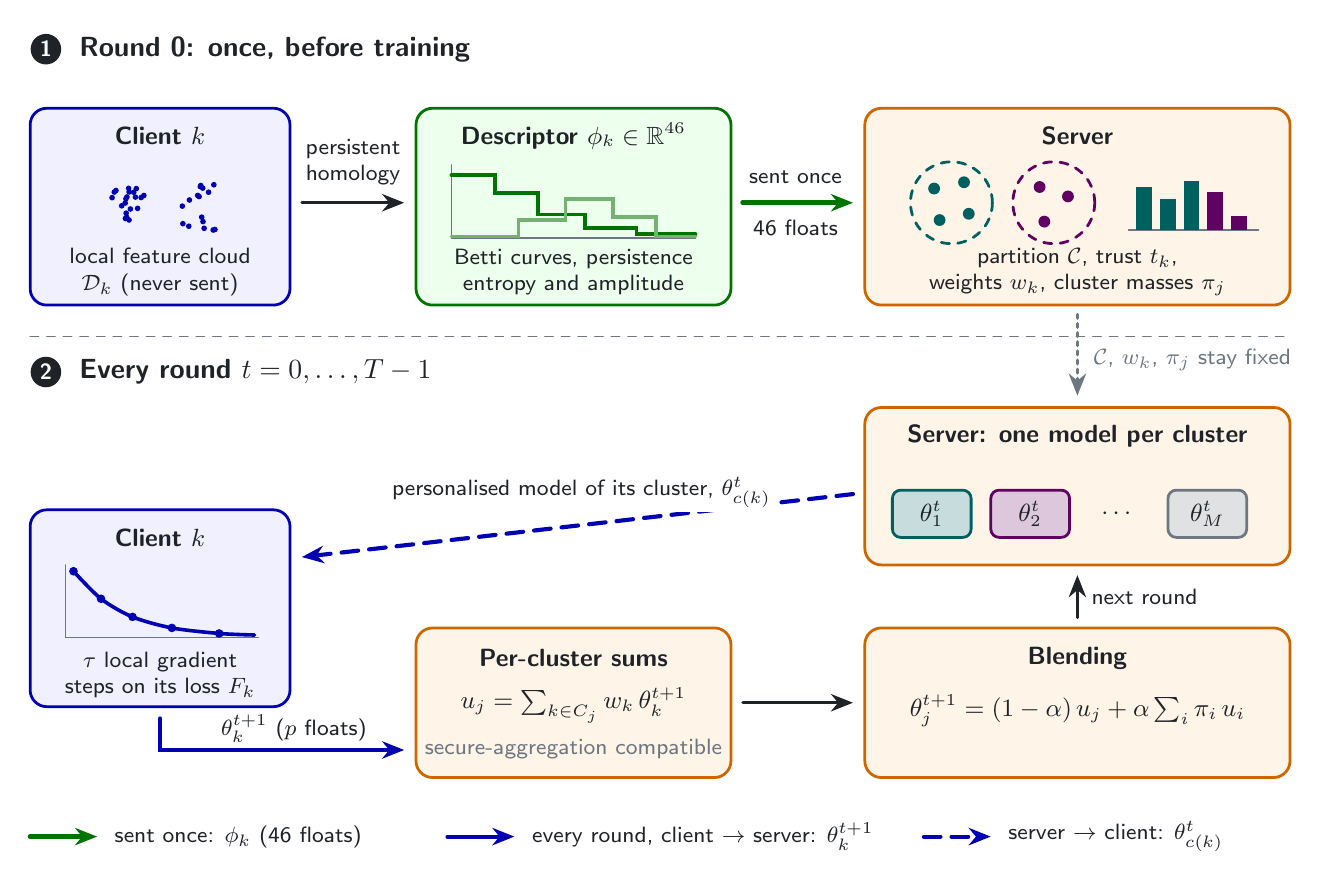
\begin{tikzpicture}[color=fg, font=\sffamily\small, line cap=round,
  >={Stealth[length=2.8mm,width=2.2mm]},
  box/.style={rounded corners=6pt, line width=1pt},
  head/.style={font=\sffamily\bfseries\small, text=fg},
  note/.style={font=\sffamily\footnotesize, text=fg, align=center},
  lab/.style={font=\sffamily\footnotesize, text=fg, fill=bg, inner sep=1.5pt, align=center},
  num/.style={circle, fill=fg, text=bg, inner sep=1.4pt, font=\sffamily\bfseries\footnotesize}]

% ============================ panel 1: round 0 ============================
\node[num] at (0.2,9.25) {1};
\node[anchor=west, font=\sffamily\bfseries\normalsize, text=fg] at (0.5,9.25) {Round 0: once, before training};

% client
\draw[box, draw=cl, fill=clfill] (0,6.0) rectangle (3.3,8.5);
\node[head] at (1.65,8.15) {Client $k$};
\pgfmathsetseed{11}
\foreach \i in {1,...,20} {\fill[cl] ({1.15+0.30*rand},{7.30+0.26*rand}) circle (0.036);}
\foreach \i in {1,...,16} {\fill[cl] ({2.15+0.22*rand},{7.25+0.32*rand}) circle (0.036);}
\node[note] at (1.65,6.42) {local feature cloud\\$\mathcal D_k$ (never sent)};

\draw[->, line width=1.1pt] (3.45,7.3) -- (4.75,7.3);
\node[note] at (4.1,7.82) {persistent\\homology};

% descriptor
\draw[box, draw=ds, fill=dsfill] (4.9,6.0) rectangle (8.9,8.5);
\node[head] at (6.9,8.15) {Descriptor $\phi_k\in\mathbb{R}^{46}$};
\draw[muted, line width=0.6pt] (5.35,6.85) -- (8.45,6.85);
\draw[muted, line width=0.6pt] (5.35,6.85) -- (5.35,7.78);
\draw[ds, line width=1.3pt] (5.35,7.65) -- (5.9,7.65) -- (5.9,7.42) -- (6.45,7.42) -- (6.45,7.15) -- (7.05,7.15)
      -- (7.05,6.98) -- (7.7,6.98) -- (7.7,6.9) -- (8.45,6.9);
\draw[ds!55!bg, line width=1.3pt] (5.35,6.87) -- (6.2,6.87) -- (6.2,7.08) -- (6.8,7.08) -- (6.8,7.35) -- (7.4,7.35)
      -- (7.4,7.12) -- (7.95,7.12) -- (7.95,6.87) -- (8.45,6.87);
\node[note] at (6.9,6.42) {Betti curves, persistence\\entropy and amplitude};

\draw[->, line width=1.8pt, draw=ds] (9.05,7.3) -- (10.45,7.3);
\node[lab] at (9.72,7.62) {sent once};
\node[lab] at (9.72,6.98) {46 floats};

% server structure
\draw[box, draw=sv, fill=svfill] (10.6,6.0) rectangle (16.0,8.5);
\node[head] at (13.3,8.15) {Server};
\draw[ca, dashed, line width=1pt] (11.7,7.3) circle (0.52);
\draw[cb, dashed, line width=1pt] (13.0,7.3) circle (0.52);
\foreach \p in {(11.48,7.48),(11.86,7.56),(11.55,7.08),(11.92,7.16)} \fill[ca] \p circle (0.075);
\foreach \p in {(12.82,7.5),(13.18,7.38),(12.88,7.06)} \fill[cb] \p circle (0.075);
\draw[muted, line width=0.6pt] (13.95,6.95) -- (15.6,6.95);
\foreach \x/\h/\c in {14.15/0.55/ca, 14.45/0.40/ca, 14.75/0.62/ca, 15.05/0.48/cb, 15.35/0.18/cb}
  \fill[\c] (\x-0.1,6.95) rectangle (\x+0.1,6.95+\h);
\node[note] at (13.3,6.42) {partition $\mathcal C$, trust $t_k$,\\weights $w_k$, cluster masses $\pi_j$};

% ============================ separator ============================
\draw[muted, dashed, line width=0.6pt] (0,5.6) -- (16,5.6);
\draw[->, muted, dotted, line width=1.3pt] (13.3,5.88) -- (13.3,4.85);
\node[lab, anchor=west, text=muted] at (13.45,5.3) {$\mathcal C$, $w_k$, $\pi_j$ stay fixed};

% ============================ panel 2: every round ============================
\node[num] at (0.2,5.15) {2};
\node[anchor=west, font=\sffamily\bfseries\normalsize, text=fg] at (0.5,5.15) {Every round $t=0,\dots,T-1$};

% server models
\draw[box, draw=sv, fill=svfill] (10.6,2.7) rectangle (16.0,4.7);
\node[head] at (13.3,4.33) {Server: one model per cluster};
\foreach \x/\c/\t in {11.45/ca/1, 12.7/cb/2, 14.95/muted/M}
  {\draw[\c, fill=\c!22!bg, rounded corners=3pt, line width=1pt] (\x-0.5,3.05) rectangle (\x+0.5,3.65);
   \node[text=fg] at (\x,3.35) {$\theta^{t}_{\t}$};}
\node[text=fg] at (13.82,3.35) {$\cdots$};

% client training
\draw[box, draw=cl, fill=clfill] (0,0.9) rectangle (3.3,3.4);
\node[head] at (1.65,3.05) {Client $k$};
\draw[muted, line width=0.6pt] (0.45,1.78) -- (2.9,1.78);
\draw[muted, line width=0.6pt] (0.45,1.78) -- (0.45,2.7);
\draw[cl, line width=1.3pt] plot[smooth] coordinates {(0.55,2.62) (0.9,2.27) (1.3,2.04) (1.8,1.9) (2.4,1.83) (2.85,1.81)};
\foreach \p in {(0.55,2.62),(0.9,2.27),(1.3,2.04),(1.8,1.9),(2.4,1.83)} \fill[cl] \p circle (0.055);
\node[note] at (1.65,1.3) {$\tau$ local gradient\\steps on its loss $F_k$};

% broadcast (dashed) and upload (solid)
\draw[->, line width=1.5pt, draw=cl, dash pattern=on 6pt off 4pt] (10.45,3.6) -- (3.45,2.8);
\node[lab] at (7.0,3.62) {personalised model of its cluster, $\theta^{t}_{c(k)}$};
\draw[->, line width=1.5pt, draw=cl] (1.65,0.75) |- (4.75,0.35);
\node[lab] at (3.35,0.62) {$\theta^{t+1}_k$ ($p$ floats)};

% aggregation and blending
\draw[box, draw=sv, fill=svfill] (4.9,0) rectangle (8.9,1.9);
\node[head] at (6.9,1.52) {Per-cluster sums};
\node[text=fg] at (6.9,0.92) {$u_j=\sum_{k\in C_j} w_k\,\theta^{t+1}_k$};
\node[note, text=muted] at (6.9,0.36) {secure-aggregation compatible};
\draw[->, line width=1.1pt] (9.05,0.95) -- (10.45,0.95);
\draw[box, draw=sv, fill=svfill] (10.6,0) rectangle (16.0,1.9);
\node[head] at (13.3,1.52) {Blending};
\node[text=fg] at (13.3,0.85) {$\theta^{t+1}_j=(1-\alpha)\,u_j+\alpha\sum_i\pi_i\,u_i$};
\draw[->, line width=1.1pt] (13.3,2.03) -- (13.3,2.57);
\node[lab, anchor=west] at (13.42,2.3) {next round};

% ============================ legend ============================
\draw[->, line width=1.8pt, draw=ds] (0,-0.75) -- (0.85,-0.75);
\node[anchor=west, font=\sffamily\footnotesize] at (0.95,-0.75) {sent once: $\phi_k$ (46 floats)};
\draw[->, line width=1.5pt, draw=cl] (5.3,-0.75) -- (6.15,-0.75);
\node[anchor=west, font=\sffamily\footnotesize] at (6.25,-0.75) {every round, client $\to$ server: $\theta^{t+1}_k$};
\draw[->, line width=1.5pt, draw=cl, dash pattern=on 6pt off 4pt] (11.35,-0.75) -- (12.2,-0.75);
\node[anchor=west, font=\sffamily\footnotesize] at (12.3,-0.75) {server $\to$ client: $\theta^{t}_{c(k)}$};
\end{tikzpicture}
\end{document}
"
%   pdflatex -jobname=ptopofl_protocol_dark  "\def\isdark{1}% pTopoFL protocol figure for the README.  Build:
%   pdflatex -jobname=ptopofl_protocol_light "\def\isdark{0}% pTopoFL protocol figure for the README.  Build:
%   pdflatex -jobname=ptopofl_protocol_light "\def\isdark{0}\input{ptopofl_protocol}"
%   pdflatex -jobname=ptopofl_protocol_dark  "\def\isdark{1}\input{ptopofl_protocol}"
%   pdftocairo -svg <name>.pdf <name>.svg   (and pdftoppm -png -r 300 -singlefile <name>.pdf <name>)
\documentclass[border=14pt]{standalone}
\usepackage{amsmath,amssymb}
\usepackage[scaled=0.92]{helvet}
\renewcommand{\familydefault}{\sfdefault}
\usepackage{tikz}
\usetikzlibrary{arrows.meta,calc}
\providecommand{\isdark}{0}
\ifnum\isdark=1
  \definecolor{bg}{HTML}{0D1117}\definecolor{fg}{HTML}{E6EDF3}\definecolor{muted}{HTML}{8B949E}
  \colorlet{cl}{blue!35!white}\colorlet{clfill}{blue!16!bg}
  \colorlet{ds}{green!65!white}\colorlet{dsfill}{green!12!bg}
  \colorlet{sv}{orange!80!white}\colorlet{svfill}{orange!13!bg}
  \colorlet{ca}{cyan!75!white}\colorlet{cb}{magenta!55!white}
\else
  \definecolor{bg}{HTML}{FFFFFF}\definecolor{fg}{HTML}{1F2328}\definecolor{muted}{HTML}{6E7781}
  \colorlet{cl}{blue!70!black}\colorlet{clfill}{blue!6}
  \colorlet{ds}{green!45!black}\colorlet{dsfill}{green!7}
  \colorlet{sv}{orange!80!black}\colorlet{svfill}{orange!9}
  \colorlet{ca}{teal!75!black}\colorlet{cb}{violet!75!black}
\fi
\pagecolor{bg}
\begin{document}
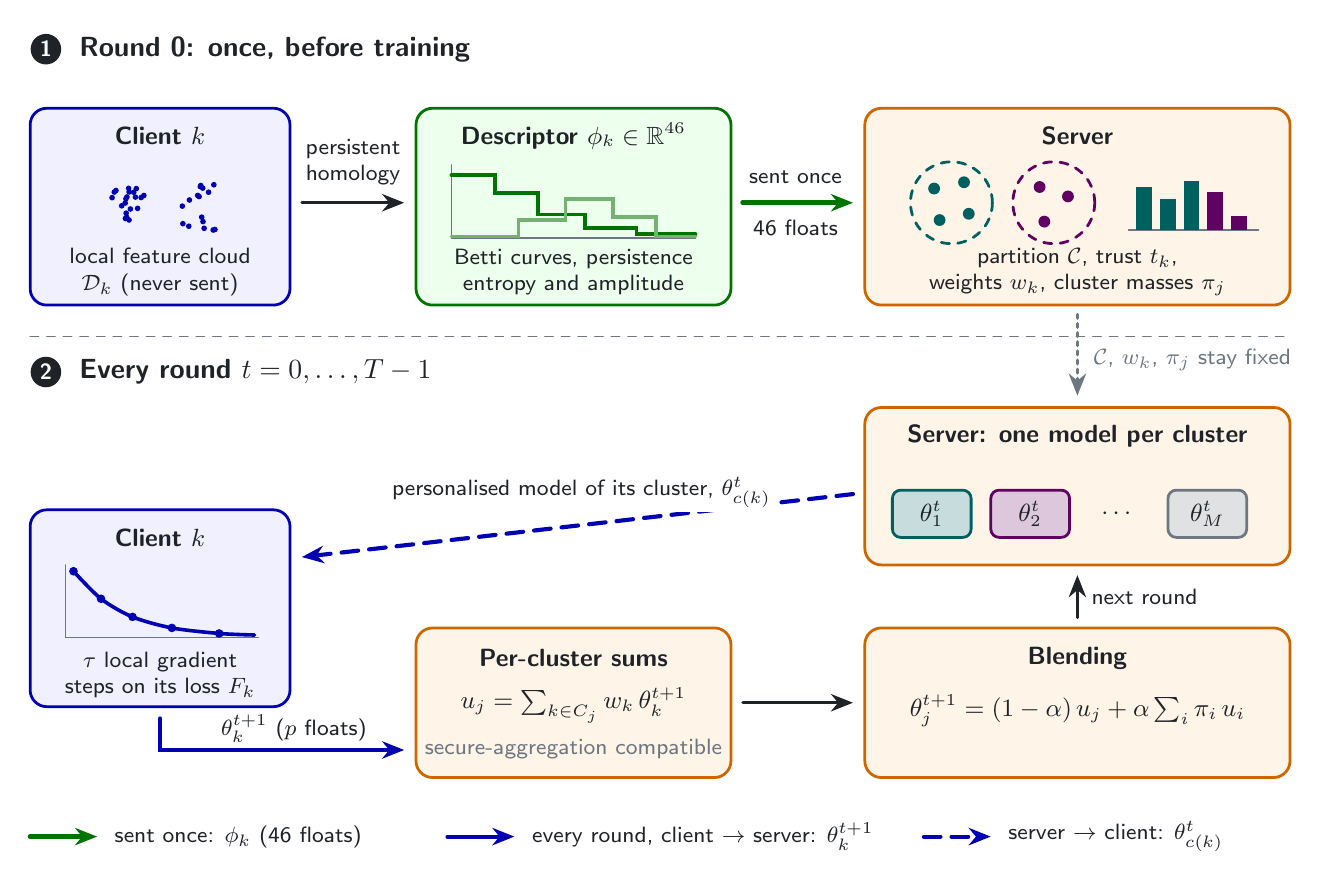
\begin{tikzpicture}[color=fg, font=\sffamily\small, line cap=round,
  >={Stealth[length=2.8mm,width=2.2mm]},
  box/.style={rounded corners=6pt, line width=1pt},
  head/.style={font=\sffamily\bfseries\small, text=fg},
  note/.style={font=\sffamily\footnotesize, text=fg, align=center},
  lab/.style={font=\sffamily\footnotesize, text=fg, fill=bg, inner sep=1.5pt, align=center},
  num/.style={circle, fill=fg, text=bg, inner sep=1.4pt, font=\sffamily\bfseries\footnotesize}]

% ============================ panel 1: round 0 ============================
\node[num] at (0.2,9.25) {1};
\node[anchor=west, font=\sffamily\bfseries\normalsize, text=fg] at (0.5,9.25) {Round 0: once, before training};

% client
\draw[box, draw=cl, fill=clfill] (0,6.0) rectangle (3.3,8.5);
\node[head] at (1.65,8.15) {Client $k$};
\pgfmathsetseed{11}
\foreach \i in {1,...,20} {\fill[cl] ({1.15+0.30*rand},{7.30+0.26*rand}) circle (0.036);}
\foreach \i in {1,...,16} {\fill[cl] ({2.15+0.22*rand},{7.25+0.32*rand}) circle (0.036);}
\node[note] at (1.65,6.42) {local feature cloud\\$\mathcal D_k$ (never sent)};

\draw[->, line width=1.1pt] (3.45,7.3) -- (4.75,7.3);
\node[note] at (4.1,7.82) {persistent\\homology};

% descriptor
\draw[box, draw=ds, fill=dsfill] (4.9,6.0) rectangle (8.9,8.5);
\node[head] at (6.9,8.15) {Descriptor $\phi_k\in\mathbb{R}^{46}$};
\draw[muted, line width=0.6pt] (5.35,6.85) -- (8.45,6.85);
\draw[muted, line width=0.6pt] (5.35,6.85) -- (5.35,7.78);
\draw[ds, line width=1.3pt] (5.35,7.65) -- (5.9,7.65) -- (5.9,7.42) -- (6.45,7.42) -- (6.45,7.15) -- (7.05,7.15)
      -- (7.05,6.98) -- (7.7,6.98) -- (7.7,6.9) -- (8.45,6.9);
\draw[ds!55!bg, line width=1.3pt] (5.35,6.87) -- (6.2,6.87) -- (6.2,7.08) -- (6.8,7.08) -- (6.8,7.35) -- (7.4,7.35)
      -- (7.4,7.12) -- (7.95,7.12) -- (7.95,6.87) -- (8.45,6.87);
\node[note] at (6.9,6.42) {Betti curves, persistence\\entropy and amplitude};

\draw[->, line width=1.8pt, draw=ds] (9.05,7.3) -- (10.45,7.3);
\node[lab] at (9.72,7.62) {sent once};
\node[lab] at (9.72,6.98) {46 floats};

% server structure
\draw[box, draw=sv, fill=svfill] (10.6,6.0) rectangle (16.0,8.5);
\node[head] at (13.3,8.15) {Server};
\draw[ca, dashed, line width=1pt] (11.7,7.3) circle (0.52);
\draw[cb, dashed, line width=1pt] (13.0,7.3) circle (0.52);
\foreach \p in {(11.48,7.48),(11.86,7.56),(11.55,7.08),(11.92,7.16)} \fill[ca] \p circle (0.075);
\foreach \p in {(12.82,7.5),(13.18,7.38),(12.88,7.06)} \fill[cb] \p circle (0.075);
\draw[muted, line width=0.6pt] (13.95,6.95) -- (15.6,6.95);
\foreach \x/\h/\c in {14.15/0.55/ca, 14.45/0.40/ca, 14.75/0.62/ca, 15.05/0.48/cb, 15.35/0.18/cb}
  \fill[\c] (\x-0.1,6.95) rectangle (\x+0.1,6.95+\h);
\node[note] at (13.3,6.42) {partition $\mathcal C$, trust $t_k$,\\weights $w_k$, cluster masses $\pi_j$};

% ============================ separator ============================
\draw[muted, dashed, line width=0.6pt] (0,5.6) -- (16,5.6);
\draw[->, muted, dotted, line width=1.3pt] (13.3,5.88) -- (13.3,4.85);
\node[lab, anchor=west, text=muted] at (13.45,5.3) {$\mathcal C$, $w_k$, $\pi_j$ stay fixed};

% ============================ panel 2: every round ============================
\node[num] at (0.2,5.15) {2};
\node[anchor=west, font=\sffamily\bfseries\normalsize, text=fg] at (0.5,5.15) {Every round $t=0,\dots,T-1$};

% server models
\draw[box, draw=sv, fill=svfill] (10.6,2.7) rectangle (16.0,4.7);
\node[head] at (13.3,4.33) {Server: one model per cluster};
\foreach \x/\c/\t in {11.45/ca/1, 12.7/cb/2, 14.95/muted/M}
  {\draw[\c, fill=\c!22!bg, rounded corners=3pt, line width=1pt] (\x-0.5,3.05) rectangle (\x+0.5,3.65);
   \node[text=fg] at (\x,3.35) {$\theta^{t}_{\t}$};}
\node[text=fg] at (13.82,3.35) {$\cdots$};

% client training
\draw[box, draw=cl, fill=clfill] (0,0.9) rectangle (3.3,3.4);
\node[head] at (1.65,3.05) {Client $k$};
\draw[muted, line width=0.6pt] (0.45,1.78) -- (2.9,1.78);
\draw[muted, line width=0.6pt] (0.45,1.78) -- (0.45,2.7);
\draw[cl, line width=1.3pt] plot[smooth] coordinates {(0.55,2.62) (0.9,2.27) (1.3,2.04) (1.8,1.9) (2.4,1.83) (2.85,1.81)};
\foreach \p in {(0.55,2.62),(0.9,2.27),(1.3,2.04),(1.8,1.9),(2.4,1.83)} \fill[cl] \p circle (0.055);
\node[note] at (1.65,1.3) {$\tau$ local gradient\\steps on its loss $F_k$};

% broadcast (dashed) and upload (solid)
\draw[->, line width=1.5pt, draw=cl, dash pattern=on 6pt off 4pt] (10.45,3.6) -- (3.45,2.8);
\node[lab] at (7.0,3.62) {personalised model of its cluster, $\theta^{t}_{c(k)}$};
\draw[->, line width=1.5pt, draw=cl] (1.65,0.75) |- (4.75,0.35);
\node[lab] at (3.35,0.62) {$\theta^{t+1}_k$ ($p$ floats)};

% aggregation and blending
\draw[box, draw=sv, fill=svfill] (4.9,0) rectangle (8.9,1.9);
\node[head] at (6.9,1.52) {Per-cluster sums};
\node[text=fg] at (6.9,0.92) {$u_j=\sum_{k\in C_j} w_k\,\theta^{t+1}_k$};
\node[note, text=muted] at (6.9,0.36) {secure-aggregation compatible};
\draw[->, line width=1.1pt] (9.05,0.95) -- (10.45,0.95);
\draw[box, draw=sv, fill=svfill] (10.6,0) rectangle (16.0,1.9);
\node[head] at (13.3,1.52) {Blending};
\node[text=fg] at (13.3,0.85) {$\theta^{t+1}_j=(1-\alpha)\,u_j+\alpha\sum_i\pi_i\,u_i$};
\draw[->, line width=1.1pt] (13.3,2.03) -- (13.3,2.57);
\node[lab, anchor=west] at (13.42,2.3) {next round};

% ============================ legend ============================
\draw[->, line width=1.8pt, draw=ds] (0,-0.75) -- (0.85,-0.75);
\node[anchor=west, font=\sffamily\footnotesize] at (0.95,-0.75) {sent once: $\phi_k$ (46 floats)};
\draw[->, line width=1.5pt, draw=cl] (5.3,-0.75) -- (6.15,-0.75);
\node[anchor=west, font=\sffamily\footnotesize] at (6.25,-0.75) {every round, client $\to$ server: $\theta^{t+1}_k$};
\draw[->, line width=1.5pt, draw=cl, dash pattern=on 6pt off 4pt] (11.35,-0.75) -- (12.2,-0.75);
\node[anchor=west, font=\sffamily\footnotesize] at (12.3,-0.75) {server $\to$ client: $\theta^{t}_{c(k)}$};
\end{tikzpicture}
\end{document}
"
%   pdflatex -jobname=ptopofl_protocol_dark  "\def\isdark{1}% pTopoFL protocol figure for the README.  Build:
%   pdflatex -jobname=ptopofl_protocol_light "\def\isdark{0}\input{ptopofl_protocol}"
%   pdflatex -jobname=ptopofl_protocol_dark  "\def\isdark{1}\input{ptopofl_protocol}"
%   pdftocairo -svg <name>.pdf <name>.svg   (and pdftoppm -png -r 300 -singlefile <name>.pdf <name>)
\documentclass[border=14pt]{standalone}
\usepackage{amsmath,amssymb}
\usepackage[scaled=0.92]{helvet}
\renewcommand{\familydefault}{\sfdefault}
\usepackage{tikz}
\usetikzlibrary{arrows.meta,calc}
\providecommand{\isdark}{0}
\ifnum\isdark=1
  \definecolor{bg}{HTML}{0D1117}\definecolor{fg}{HTML}{E6EDF3}\definecolor{muted}{HTML}{8B949E}
  \colorlet{cl}{blue!35!white}\colorlet{clfill}{blue!16!bg}
  \colorlet{ds}{green!65!white}\colorlet{dsfill}{green!12!bg}
  \colorlet{sv}{orange!80!white}\colorlet{svfill}{orange!13!bg}
  \colorlet{ca}{cyan!75!white}\colorlet{cb}{magenta!55!white}
\else
  \definecolor{bg}{HTML}{FFFFFF}\definecolor{fg}{HTML}{1F2328}\definecolor{muted}{HTML}{6E7781}
  \colorlet{cl}{blue!70!black}\colorlet{clfill}{blue!6}
  \colorlet{ds}{green!45!black}\colorlet{dsfill}{green!7}
  \colorlet{sv}{orange!80!black}\colorlet{svfill}{orange!9}
  \colorlet{ca}{teal!75!black}\colorlet{cb}{violet!75!black}
\fi
\pagecolor{bg}
\begin{document}
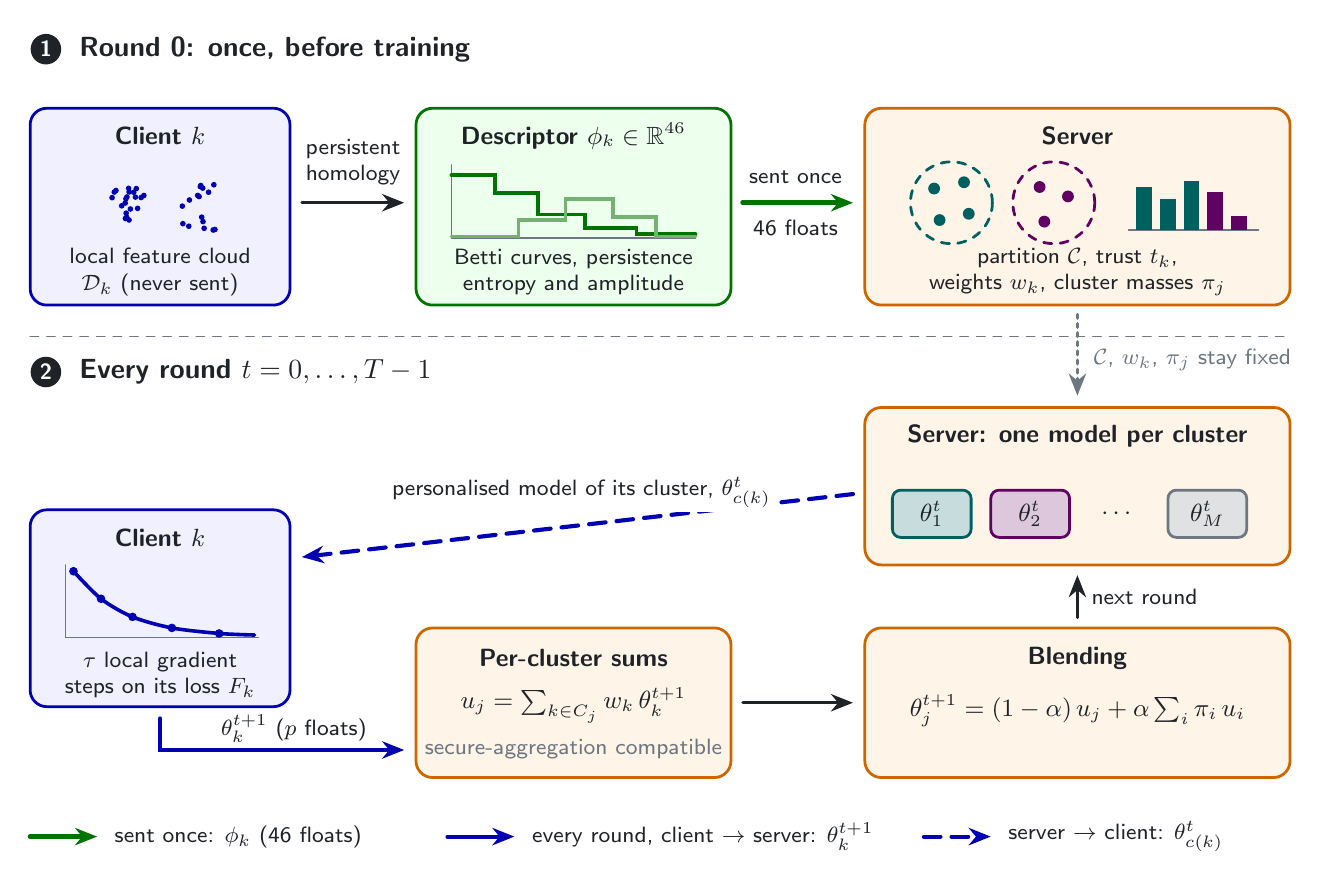
\begin{tikzpicture}[color=fg, font=\sffamily\small, line cap=round,
  >={Stealth[length=2.8mm,width=2.2mm]},
  box/.style={rounded corners=6pt, line width=1pt},
  head/.style={font=\sffamily\bfseries\small, text=fg},
  note/.style={font=\sffamily\footnotesize, text=fg, align=center},
  lab/.style={font=\sffamily\footnotesize, text=fg, fill=bg, inner sep=1.5pt, align=center},
  num/.style={circle, fill=fg, text=bg, inner sep=1.4pt, font=\sffamily\bfseries\footnotesize}]

% ============================ panel 1: round 0 ============================
\node[num] at (0.2,9.25) {1};
\node[anchor=west, font=\sffamily\bfseries\normalsize, text=fg] at (0.5,9.25) {Round 0: once, before training};

% client
\draw[box, draw=cl, fill=clfill] (0,6.0) rectangle (3.3,8.5);
\node[head] at (1.65,8.15) {Client $k$};
\pgfmathsetseed{11}
\foreach \i in {1,...,20} {\fill[cl] ({1.15+0.30*rand},{7.30+0.26*rand}) circle (0.036);}
\foreach \i in {1,...,16} {\fill[cl] ({2.15+0.22*rand},{7.25+0.32*rand}) circle (0.036);}
\node[note] at (1.65,6.42) {local feature cloud\\$\mathcal D_k$ (never sent)};

\draw[->, line width=1.1pt] (3.45,7.3) -- (4.75,7.3);
\node[note] at (4.1,7.82) {persistent\\homology};

% descriptor
\draw[box, draw=ds, fill=dsfill] (4.9,6.0) rectangle (8.9,8.5);
\node[head] at (6.9,8.15) {Descriptor $\phi_k\in\mathbb{R}^{46}$};
\draw[muted, line width=0.6pt] (5.35,6.85) -- (8.45,6.85);
\draw[muted, line width=0.6pt] (5.35,6.85) -- (5.35,7.78);
\draw[ds, line width=1.3pt] (5.35,7.65) -- (5.9,7.65) -- (5.9,7.42) -- (6.45,7.42) -- (6.45,7.15) -- (7.05,7.15)
      -- (7.05,6.98) -- (7.7,6.98) -- (7.7,6.9) -- (8.45,6.9);
\draw[ds!55!bg, line width=1.3pt] (5.35,6.87) -- (6.2,6.87) -- (6.2,7.08) -- (6.8,7.08) -- (6.8,7.35) -- (7.4,7.35)
      -- (7.4,7.12) -- (7.95,7.12) -- (7.95,6.87) -- (8.45,6.87);
\node[note] at (6.9,6.42) {Betti curves, persistence\\entropy and amplitude};

\draw[->, line width=1.8pt, draw=ds] (9.05,7.3) -- (10.45,7.3);
\node[lab] at (9.72,7.62) {sent once};
\node[lab] at (9.72,6.98) {46 floats};

% server structure
\draw[box, draw=sv, fill=svfill] (10.6,6.0) rectangle (16.0,8.5);
\node[head] at (13.3,8.15) {Server};
\draw[ca, dashed, line width=1pt] (11.7,7.3) circle (0.52);
\draw[cb, dashed, line width=1pt] (13.0,7.3) circle (0.52);
\foreach \p in {(11.48,7.48),(11.86,7.56),(11.55,7.08),(11.92,7.16)} \fill[ca] \p circle (0.075);
\foreach \p in {(12.82,7.5),(13.18,7.38),(12.88,7.06)} \fill[cb] \p circle (0.075);
\draw[muted, line width=0.6pt] (13.95,6.95) -- (15.6,6.95);
\foreach \x/\h/\c in {14.15/0.55/ca, 14.45/0.40/ca, 14.75/0.62/ca, 15.05/0.48/cb, 15.35/0.18/cb}
  \fill[\c] (\x-0.1,6.95) rectangle (\x+0.1,6.95+\h);
\node[note] at (13.3,6.42) {partition $\mathcal C$, trust $t_k$,\\weights $w_k$, cluster masses $\pi_j$};

% ============================ separator ============================
\draw[muted, dashed, line width=0.6pt] (0,5.6) -- (16,5.6);
\draw[->, muted, dotted, line width=1.3pt] (13.3,5.88) -- (13.3,4.85);
\node[lab, anchor=west, text=muted] at (13.45,5.3) {$\mathcal C$, $w_k$, $\pi_j$ stay fixed};

% ============================ panel 2: every round ============================
\node[num] at (0.2,5.15) {2};
\node[anchor=west, font=\sffamily\bfseries\normalsize, text=fg] at (0.5,5.15) {Every round $t=0,\dots,T-1$};

% server models
\draw[box, draw=sv, fill=svfill] (10.6,2.7) rectangle (16.0,4.7);
\node[head] at (13.3,4.33) {Server: one model per cluster};
\foreach \x/\c/\t in {11.45/ca/1, 12.7/cb/2, 14.95/muted/M}
  {\draw[\c, fill=\c!22!bg, rounded corners=3pt, line width=1pt] (\x-0.5,3.05) rectangle (\x+0.5,3.65);
   \node[text=fg] at (\x,3.35) {$\theta^{t}_{\t}$};}
\node[text=fg] at (13.82,3.35) {$\cdots$};

% client training
\draw[box, draw=cl, fill=clfill] (0,0.9) rectangle (3.3,3.4);
\node[head] at (1.65,3.05) {Client $k$};
\draw[muted, line width=0.6pt] (0.45,1.78) -- (2.9,1.78);
\draw[muted, line width=0.6pt] (0.45,1.78) -- (0.45,2.7);
\draw[cl, line width=1.3pt] plot[smooth] coordinates {(0.55,2.62) (0.9,2.27) (1.3,2.04) (1.8,1.9) (2.4,1.83) (2.85,1.81)};
\foreach \p in {(0.55,2.62),(0.9,2.27),(1.3,2.04),(1.8,1.9),(2.4,1.83)} \fill[cl] \p circle (0.055);
\node[note] at (1.65,1.3) {$\tau$ local gradient\\steps on its loss $F_k$};

% broadcast (dashed) and upload (solid)
\draw[->, line width=1.5pt, draw=cl, dash pattern=on 6pt off 4pt] (10.45,3.6) -- (3.45,2.8);
\node[lab] at (7.0,3.62) {personalised model of its cluster, $\theta^{t}_{c(k)}$};
\draw[->, line width=1.5pt, draw=cl] (1.65,0.75) |- (4.75,0.35);
\node[lab] at (3.35,0.62) {$\theta^{t+1}_k$ ($p$ floats)};

% aggregation and blending
\draw[box, draw=sv, fill=svfill] (4.9,0) rectangle (8.9,1.9);
\node[head] at (6.9,1.52) {Per-cluster sums};
\node[text=fg] at (6.9,0.92) {$u_j=\sum_{k\in C_j} w_k\,\theta^{t+1}_k$};
\node[note, text=muted] at (6.9,0.36) {secure-aggregation compatible};
\draw[->, line width=1.1pt] (9.05,0.95) -- (10.45,0.95);
\draw[box, draw=sv, fill=svfill] (10.6,0) rectangle (16.0,1.9);
\node[head] at (13.3,1.52) {Blending};
\node[text=fg] at (13.3,0.85) {$\theta^{t+1}_j=(1-\alpha)\,u_j+\alpha\sum_i\pi_i\,u_i$};
\draw[->, line width=1.1pt] (13.3,2.03) -- (13.3,2.57);
\node[lab, anchor=west] at (13.42,2.3) {next round};

% ============================ legend ============================
\draw[->, line width=1.8pt, draw=ds] (0,-0.75) -- (0.85,-0.75);
\node[anchor=west, font=\sffamily\footnotesize] at (0.95,-0.75) {sent once: $\phi_k$ (46 floats)};
\draw[->, line width=1.5pt, draw=cl] (5.3,-0.75) -- (6.15,-0.75);
\node[anchor=west, font=\sffamily\footnotesize] at (6.25,-0.75) {every round, client $\to$ server: $\theta^{t+1}_k$};
\draw[->, line width=1.5pt, draw=cl, dash pattern=on 6pt off 4pt] (11.35,-0.75) -- (12.2,-0.75);
\node[anchor=west, font=\sffamily\footnotesize] at (12.3,-0.75) {server $\to$ client: $\theta^{t}_{c(k)}$};
\end{tikzpicture}
\end{document}
"
%   pdftocairo -svg <name>.pdf <name>.svg   (and pdftoppm -png -r 300 -singlefile <name>.pdf <name>)
\documentclass[border=14pt]{standalone}
\usepackage{amsmath,amssymb}
\usepackage[scaled=0.92]{helvet}
\renewcommand{\familydefault}{\sfdefault}
\usepackage{tikz}
\usetikzlibrary{arrows.meta,calc}
\providecommand{\isdark}{0}
\ifnum\isdark=1
  \definecolor{bg}{HTML}{0D1117}\definecolor{fg}{HTML}{E6EDF3}\definecolor{muted}{HTML}{8B949E}
  \colorlet{cl}{blue!35!white}\colorlet{clfill}{blue!16!bg}
  \colorlet{ds}{green!65!white}\colorlet{dsfill}{green!12!bg}
  \colorlet{sv}{orange!80!white}\colorlet{svfill}{orange!13!bg}
  \colorlet{ca}{cyan!75!white}\colorlet{cb}{magenta!55!white}
\else
  \definecolor{bg}{HTML}{FFFFFF}\definecolor{fg}{HTML}{1F2328}\definecolor{muted}{HTML}{6E7781}
  \colorlet{cl}{blue!70!black}\colorlet{clfill}{blue!6}
  \colorlet{ds}{green!45!black}\colorlet{dsfill}{green!7}
  \colorlet{sv}{orange!80!black}\colorlet{svfill}{orange!9}
  \colorlet{ca}{teal!75!black}\colorlet{cb}{violet!75!black}
\fi
\pagecolor{bg}
\begin{document}
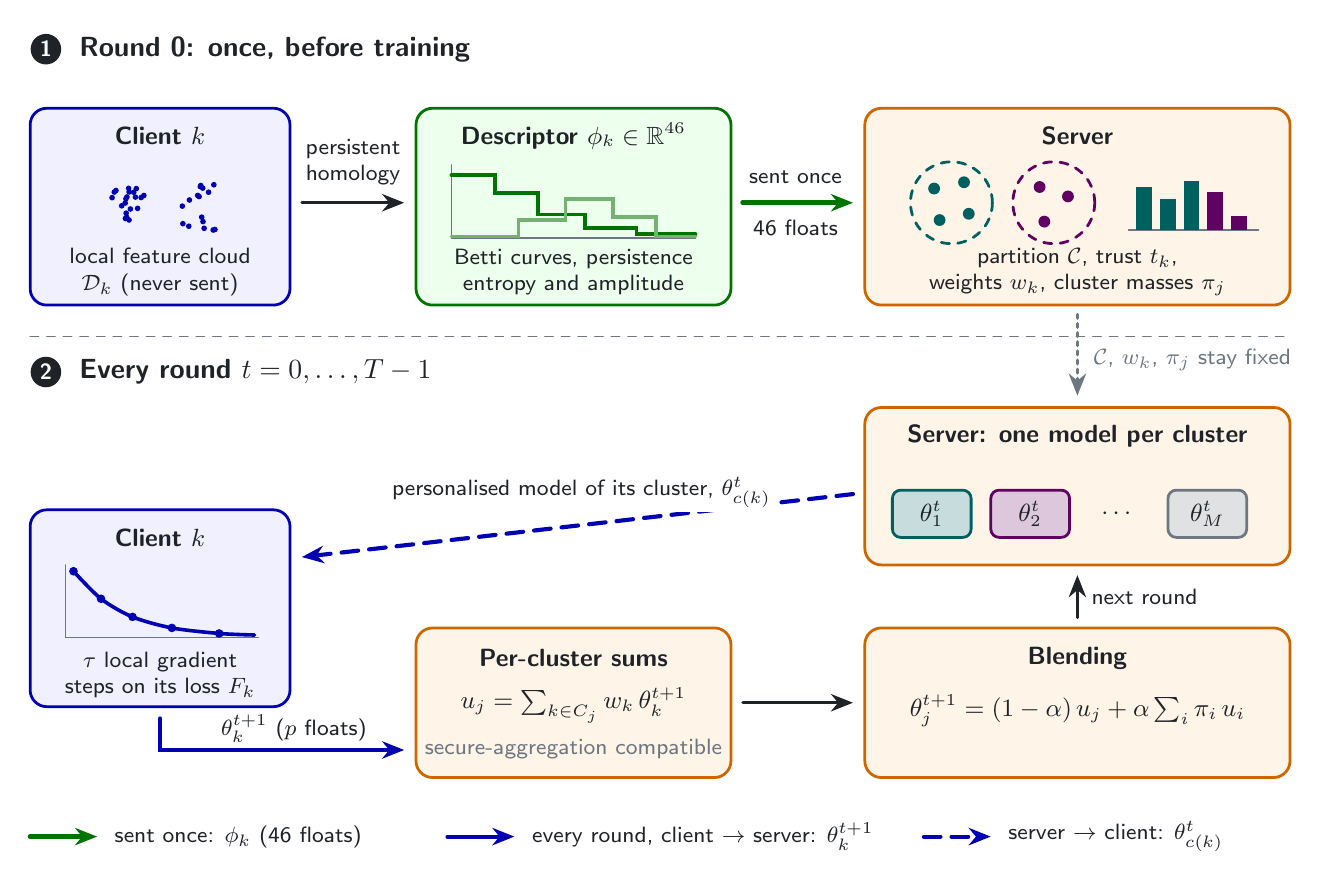
\begin{tikzpicture}[color=fg, font=\sffamily\small, line cap=round,
  >={Stealth[length=2.8mm,width=2.2mm]},
  box/.style={rounded corners=6pt, line width=1pt},
  head/.style={font=\sffamily\bfseries\small, text=fg},
  note/.style={font=\sffamily\footnotesize, text=fg, align=center},
  lab/.style={font=\sffamily\footnotesize, text=fg, fill=bg, inner sep=1.5pt, align=center},
  num/.style={circle, fill=fg, text=bg, inner sep=1.4pt, font=\sffamily\bfseries\footnotesize}]

% ============================ panel 1: round 0 ============================
\node[num] at (0.2,9.25) {1};
\node[anchor=west, font=\sffamily\bfseries\normalsize, text=fg] at (0.5,9.25) {Round 0: once, before training};

% client
\draw[box, draw=cl, fill=clfill] (0,6.0) rectangle (3.3,8.5);
\node[head] at (1.65,8.15) {Client $k$};
\pgfmathsetseed{11}
\foreach \i in {1,...,20} {\fill[cl] ({1.15+0.30*rand},{7.30+0.26*rand}) circle (0.036);}
\foreach \i in {1,...,16} {\fill[cl] ({2.15+0.22*rand},{7.25+0.32*rand}) circle (0.036);}
\node[note] at (1.65,6.42) {local feature cloud\\$\mathcal D_k$ (never sent)};

\draw[->, line width=1.1pt] (3.45,7.3) -- (4.75,7.3);
\node[note] at (4.1,7.82) {persistent\\homology};

% descriptor
\draw[box, draw=ds, fill=dsfill] (4.9,6.0) rectangle (8.9,8.5);
\node[head] at (6.9,8.15) {Descriptor $\phi_k\in\mathbb{R}^{46}$};
\draw[muted, line width=0.6pt] (5.35,6.85) -- (8.45,6.85);
\draw[muted, line width=0.6pt] (5.35,6.85) -- (5.35,7.78);
\draw[ds, line width=1.3pt] (5.35,7.65) -- (5.9,7.65) -- (5.9,7.42) -- (6.45,7.42) -- (6.45,7.15) -- (7.05,7.15)
      -- (7.05,6.98) -- (7.7,6.98) -- (7.7,6.9) -- (8.45,6.9);
\draw[ds!55!bg, line width=1.3pt] (5.35,6.87) -- (6.2,6.87) -- (6.2,7.08) -- (6.8,7.08) -- (6.8,7.35) -- (7.4,7.35)
      -- (7.4,7.12) -- (7.95,7.12) -- (7.95,6.87) -- (8.45,6.87);
\node[note] at (6.9,6.42) {Betti curves, persistence\\entropy and amplitude};

\draw[->, line width=1.8pt, draw=ds] (9.05,7.3) -- (10.45,7.3);
\node[lab] at (9.72,7.62) {sent once};
\node[lab] at (9.72,6.98) {46 floats};

% server structure
\draw[box, draw=sv, fill=svfill] (10.6,6.0) rectangle (16.0,8.5);
\node[head] at (13.3,8.15) {Server};
\draw[ca, dashed, line width=1pt] (11.7,7.3) circle (0.52);
\draw[cb, dashed, line width=1pt] (13.0,7.3) circle (0.52);
\foreach \p in {(11.48,7.48),(11.86,7.56),(11.55,7.08),(11.92,7.16)} \fill[ca] \p circle (0.075);
\foreach \p in {(12.82,7.5),(13.18,7.38),(12.88,7.06)} \fill[cb] \p circle (0.075);
\draw[muted, line width=0.6pt] (13.95,6.95) -- (15.6,6.95);
\foreach \x/\h/\c in {14.15/0.55/ca, 14.45/0.40/ca, 14.75/0.62/ca, 15.05/0.48/cb, 15.35/0.18/cb}
  \fill[\c] (\x-0.1,6.95) rectangle (\x+0.1,6.95+\h);
\node[note] at (13.3,6.42) {partition $\mathcal C$, trust $t_k$,\\weights $w_k$, cluster masses $\pi_j$};

% ============================ separator ============================
\draw[muted, dashed, line width=0.6pt] (0,5.6) -- (16,5.6);
\draw[->, muted, dotted, line width=1.3pt] (13.3,5.88) -- (13.3,4.85);
\node[lab, anchor=west, text=muted] at (13.45,5.3) {$\mathcal C$, $w_k$, $\pi_j$ stay fixed};

% ============================ panel 2: every round ============================
\node[num] at (0.2,5.15) {2};
\node[anchor=west, font=\sffamily\bfseries\normalsize, text=fg] at (0.5,5.15) {Every round $t=0,\dots,T-1$};

% server models
\draw[box, draw=sv, fill=svfill] (10.6,2.7) rectangle (16.0,4.7);
\node[head] at (13.3,4.33) {Server: one model per cluster};
\foreach \x/\c/\t in {11.45/ca/1, 12.7/cb/2, 14.95/muted/M}
  {\draw[\c, fill=\c!22!bg, rounded corners=3pt, line width=1pt] (\x-0.5,3.05) rectangle (\x+0.5,3.65);
   \node[text=fg] at (\x,3.35) {$\theta^{t}_{\t}$};}
\node[text=fg] at (13.82,3.35) {$\cdots$};

% client training
\draw[box, draw=cl, fill=clfill] (0,0.9) rectangle (3.3,3.4);
\node[head] at (1.65,3.05) {Client $k$};
\draw[muted, line width=0.6pt] (0.45,1.78) -- (2.9,1.78);
\draw[muted, line width=0.6pt] (0.45,1.78) -- (0.45,2.7);
\draw[cl, line width=1.3pt] plot[smooth] coordinates {(0.55,2.62) (0.9,2.27) (1.3,2.04) (1.8,1.9) (2.4,1.83) (2.85,1.81)};
\foreach \p in {(0.55,2.62),(0.9,2.27),(1.3,2.04),(1.8,1.9),(2.4,1.83)} \fill[cl] \p circle (0.055);
\node[note] at (1.65,1.3) {$\tau$ local gradient\\steps on its loss $F_k$};

% broadcast (dashed) and upload (solid)
\draw[->, line width=1.5pt, draw=cl, dash pattern=on 6pt off 4pt] (10.45,3.6) -- (3.45,2.8);
\node[lab] at (7.0,3.62) {personalised model of its cluster, $\theta^{t}_{c(k)}$};
\draw[->, line width=1.5pt, draw=cl] (1.65,0.75) |- (4.75,0.35);
\node[lab] at (3.35,0.62) {$\theta^{t+1}_k$ ($p$ floats)};

% aggregation and blending
\draw[box, draw=sv, fill=svfill] (4.9,0) rectangle (8.9,1.9);
\node[head] at (6.9,1.52) {Per-cluster sums};
\node[text=fg] at (6.9,0.92) {$u_j=\sum_{k\in C_j} w_k\,\theta^{t+1}_k$};
\node[note, text=muted] at (6.9,0.36) {secure-aggregation compatible};
\draw[->, line width=1.1pt] (9.05,0.95) -- (10.45,0.95);
\draw[box, draw=sv, fill=svfill] (10.6,0) rectangle (16.0,1.9);
\node[head] at (13.3,1.52) {Blending};
\node[text=fg] at (13.3,0.85) {$\theta^{t+1}_j=(1-\alpha)\,u_j+\alpha\sum_i\pi_i\,u_i$};
\draw[->, line width=1.1pt] (13.3,2.03) -- (13.3,2.57);
\node[lab, anchor=west] at (13.42,2.3) {next round};

% ============================ legend ============================
\draw[->, line width=1.8pt, draw=ds] (0,-0.75) -- (0.85,-0.75);
\node[anchor=west, font=\sffamily\footnotesize] at (0.95,-0.75) {sent once: $\phi_k$ (46 floats)};
\draw[->, line width=1.5pt, draw=cl] (5.3,-0.75) -- (6.15,-0.75);
\node[anchor=west, font=\sffamily\footnotesize] at (6.25,-0.75) {every round, client $\to$ server: $\theta^{t+1}_k$};
\draw[->, line width=1.5pt, draw=cl, dash pattern=on 6pt off 4pt] (11.35,-0.75) -- (12.2,-0.75);
\node[anchor=west, font=\sffamily\footnotesize] at (12.3,-0.75) {server $\to$ client: $\theta^{t}_{c(k)}$};
\end{tikzpicture}
\end{document}
"
%   pdftocairo -svg <name>.pdf <name>.svg   (and pdftoppm -png -r 300 -singlefile <name>.pdf <name>)
\documentclass[border=14pt]{standalone}
\usepackage{amsmath,amssymb}
\usepackage[scaled=0.92]{helvet}
\renewcommand{\familydefault}{\sfdefault}
\usepackage{tikz}
\usetikzlibrary{arrows.meta,calc}
\providecommand{\isdark}{0}
\ifnum\isdark=1
  \definecolor{bg}{HTML}{0D1117}\definecolor{fg}{HTML}{E6EDF3}\definecolor{muted}{HTML}{8B949E}
  \colorlet{cl}{blue!35!white}\colorlet{clfill}{blue!16!bg}
  \colorlet{ds}{green!65!white}\colorlet{dsfill}{green!12!bg}
  \colorlet{sv}{orange!80!white}\colorlet{svfill}{orange!13!bg}
  \colorlet{ca}{cyan!75!white}\colorlet{cb}{magenta!55!white}
\else
  \definecolor{bg}{HTML}{FFFFFF}\definecolor{fg}{HTML}{1F2328}\definecolor{muted}{HTML}{6E7781}
  \colorlet{cl}{blue!70!black}\colorlet{clfill}{blue!6}
  \colorlet{ds}{green!45!black}\colorlet{dsfill}{green!7}
  \colorlet{sv}{orange!80!black}\colorlet{svfill}{orange!9}
  \colorlet{ca}{teal!75!black}\colorlet{cb}{violet!75!black}
\fi
\pagecolor{bg}
\begin{document}
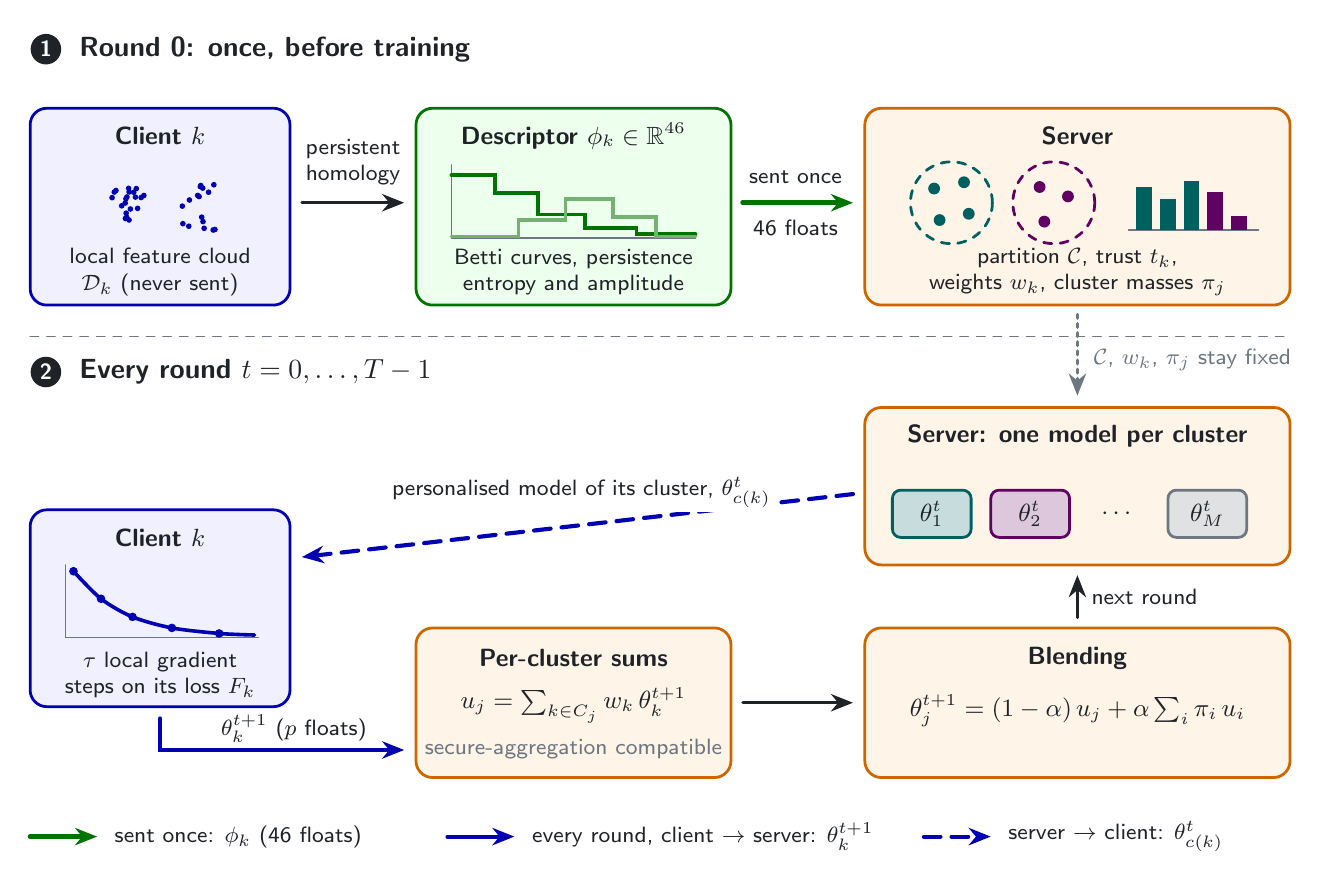
\begin{tikzpicture}[color=fg, font=\sffamily\small, line cap=round,
  >={Stealth[length=2.8mm,width=2.2mm]},
  box/.style={rounded corners=6pt, line width=1pt},
  head/.style={font=\sffamily\bfseries\small, text=fg},
  note/.style={font=\sffamily\footnotesize, text=fg, align=center},
  lab/.style={font=\sffamily\footnotesize, text=fg, fill=bg, inner sep=1.5pt, align=center},
  num/.style={circle, fill=fg, text=bg, inner sep=1.4pt, font=\sffamily\bfseries\footnotesize}]

% ============================ panel 1: round 0 ============================
\node[num] at (0.2,9.25) {1};
\node[anchor=west, font=\sffamily\bfseries\normalsize, text=fg] at (0.5,9.25) {Round 0: once, before training};

% client
\draw[box, draw=cl, fill=clfill] (0,6.0) rectangle (3.3,8.5);
\node[head] at (1.65,8.15) {Client $k$};
\pgfmathsetseed{11}
\foreach \i in {1,...,20} {\fill[cl] ({1.15+0.30*rand},{7.30+0.26*rand}) circle (0.036);}
\foreach \i in {1,...,16} {\fill[cl] ({2.15+0.22*rand},{7.25+0.32*rand}) circle (0.036);}
\node[note] at (1.65,6.42) {local feature cloud\\$\mathcal D_k$ (never sent)};

\draw[->, line width=1.1pt] (3.45,7.3) -- (4.75,7.3);
\node[note] at (4.1,7.82) {persistent\\homology};

% descriptor
\draw[box, draw=ds, fill=dsfill] (4.9,6.0) rectangle (8.9,8.5);
\node[head] at (6.9,8.15) {Descriptor $\phi_k\in\mathbb{R}^{46}$};
\draw[muted, line width=0.6pt] (5.35,6.85) -- (8.45,6.85);
\draw[muted, line width=0.6pt] (5.35,6.85) -- (5.35,7.78);
\draw[ds, line width=1.3pt] (5.35,7.65) -- (5.9,7.65) -- (5.9,7.42) -- (6.45,7.42) -- (6.45,7.15) -- (7.05,7.15)
      -- (7.05,6.98) -- (7.7,6.98) -- (7.7,6.9) -- (8.45,6.9);
\draw[ds!55!bg, line width=1.3pt] (5.35,6.87) -- (6.2,6.87) -- (6.2,7.08) -- (6.8,7.08) -- (6.8,7.35) -- (7.4,7.35)
      -- (7.4,7.12) -- (7.95,7.12) -- (7.95,6.87) -- (8.45,6.87);
\node[note] at (6.9,6.42) {Betti curves, persistence\\entropy and amplitude};

\draw[->, line width=1.8pt, draw=ds] (9.05,7.3) -- (10.45,7.3);
\node[lab] at (9.72,7.62) {sent once};
\node[lab] at (9.72,6.98) {46 floats};

% server structure
\draw[box, draw=sv, fill=svfill] (10.6,6.0) rectangle (16.0,8.5);
\node[head] at (13.3,8.15) {Server};
\draw[ca, dashed, line width=1pt] (11.7,7.3) circle (0.52);
\draw[cb, dashed, line width=1pt] (13.0,7.3) circle (0.52);
\foreach \p in {(11.48,7.48),(11.86,7.56),(11.55,7.08),(11.92,7.16)} \fill[ca] \p circle (0.075);
\foreach \p in {(12.82,7.5),(13.18,7.38),(12.88,7.06)} \fill[cb] \p circle (0.075);
\draw[muted, line width=0.6pt] (13.95,6.95) -- (15.6,6.95);
\foreach \x/\h/\c in {14.15/0.55/ca, 14.45/0.40/ca, 14.75/0.62/ca, 15.05/0.48/cb, 15.35/0.18/cb}
  \fill[\c] (\x-0.1,6.95) rectangle (\x+0.1,6.95+\h);
\node[note] at (13.3,6.42) {partition $\mathcal C$, trust $t_k$,\\weights $w_k$, cluster masses $\pi_j$};

% ============================ separator ============================
\draw[muted, dashed, line width=0.6pt] (0,5.6) -- (16,5.6);
\draw[->, muted, dotted, line width=1.3pt] (13.3,5.88) -- (13.3,4.85);
\node[lab, anchor=west, text=muted] at (13.45,5.3) {$\mathcal C$, $w_k$, $\pi_j$ stay fixed};

% ============================ panel 2: every round ============================
\node[num] at (0.2,5.15) {2};
\node[anchor=west, font=\sffamily\bfseries\normalsize, text=fg] at (0.5,5.15) {Every round $t=0,\dots,T-1$};

% server models
\draw[box, draw=sv, fill=svfill] (10.6,2.7) rectangle (16.0,4.7);
\node[head] at (13.3,4.33) {Server: one model per cluster};
\foreach \x/\c/\t in {11.45/ca/1, 12.7/cb/2, 14.95/muted/M}
  {\draw[\c, fill=\c!22!bg, rounded corners=3pt, line width=1pt] (\x-0.5,3.05) rectangle (\x+0.5,3.65);
   \node[text=fg] at (\x,3.35) {$\theta^{t}_{\t}$};}
\node[text=fg] at (13.82,3.35) {$\cdots$};

% client training
\draw[box, draw=cl, fill=clfill] (0,0.9) rectangle (3.3,3.4);
\node[head] at (1.65,3.05) {Client $k$};
\draw[muted, line width=0.6pt] (0.45,1.78) -- (2.9,1.78);
\draw[muted, line width=0.6pt] (0.45,1.78) -- (0.45,2.7);
\draw[cl, line width=1.3pt] plot[smooth] coordinates {(0.55,2.62) (0.9,2.27) (1.3,2.04) (1.8,1.9) (2.4,1.83) (2.85,1.81)};
\foreach \p in {(0.55,2.62),(0.9,2.27),(1.3,2.04),(1.8,1.9),(2.4,1.83)} \fill[cl] \p circle (0.055);
\node[note] at (1.65,1.3) {$\tau$ local gradient\\steps on its loss $F_k$};

% broadcast (dashed) and upload (solid)
\draw[->, line width=1.5pt, draw=cl, dash pattern=on 6pt off 4pt] (10.45,3.6) -- (3.45,2.8);
\node[lab] at (7.0,3.62) {personalised model of its cluster, $\theta^{t}_{c(k)}$};
\draw[->, line width=1.5pt, draw=cl] (1.65,0.75) |- (4.75,0.35);
\node[lab] at (3.35,0.62) {$\theta^{t+1}_k$ ($p$ floats)};

% aggregation and blending
\draw[box, draw=sv, fill=svfill] (4.9,0) rectangle (8.9,1.9);
\node[head] at (6.9,1.52) {Per-cluster sums};
\node[text=fg] at (6.9,0.92) {$u_j=\sum_{k\in C_j} w_k\,\theta^{t+1}_k$};
\node[note, text=muted] at (6.9,0.36) {secure-aggregation compatible};
\draw[->, line width=1.1pt] (9.05,0.95) -- (10.45,0.95);
\draw[box, draw=sv, fill=svfill] (10.6,0) rectangle (16.0,1.9);
\node[head] at (13.3,1.52) {Blending};
\node[text=fg] at (13.3,0.85) {$\theta^{t+1}_j=(1-\alpha)\,u_j+\alpha\sum_i\pi_i\,u_i$};
\draw[->, line width=1.1pt] (13.3,2.03) -- (13.3,2.57);
\node[lab, anchor=west] at (13.42,2.3) {next round};

% ============================ legend ============================
\draw[->, line width=1.8pt, draw=ds] (0,-0.75) -- (0.85,-0.75);
\node[anchor=west, font=\sffamily\footnotesize] at (0.95,-0.75) {sent once: $\phi_k$ (46 floats)};
\draw[->, line width=1.5pt, draw=cl] (5.3,-0.75) -- (6.15,-0.75);
\node[anchor=west, font=\sffamily\footnotesize] at (6.25,-0.75) {every round, client $\to$ server: $\theta^{t+1}_k$};
\draw[->, line width=1.5pt, draw=cl, dash pattern=on 6pt off 4pt] (11.35,-0.75) -- (12.2,-0.75);
\node[anchor=west, font=\sffamily\footnotesize] at (12.3,-0.75) {server $\to$ client: $\theta^{t}_{c(k)}$};
\end{tikzpicture}
\end{document}
"
%   pdftocairo -svg <name>.pdf <name>.svg   (and pdftoppm -png -r 300 -singlefile <name>.pdf <name>)
\documentclass[border=14pt]{standalone}
\usepackage{amsmath,amssymb}
\usepackage[scaled=0.92]{helvet}
\renewcommand{\familydefault}{\sfdefault}
\usepackage{tikz}
\usetikzlibrary{arrows.meta,calc}
\providecommand{\isdark}{0}
\ifnum\isdark=1
  \definecolor{bg}{HTML}{0D1117}\definecolor{fg}{HTML}{E6EDF3}\definecolor{muted}{HTML}{8B949E}
  \colorlet{cl}{blue!35!white}\colorlet{clfill}{blue!16!bg}
  \colorlet{ds}{green!65!white}\colorlet{dsfill}{green!12!bg}
  \colorlet{sv}{orange!80!white}\colorlet{svfill}{orange!13!bg}
  \colorlet{ca}{cyan!75!white}\colorlet{cb}{magenta!55!white}
\else
  \definecolor{bg}{HTML}{FFFFFF}\definecolor{fg}{HTML}{1F2328}\definecolor{muted}{HTML}{6E7781}
  \colorlet{cl}{blue!70!black}\colorlet{clfill}{blue!6}
  \colorlet{ds}{green!45!black}\colorlet{dsfill}{green!7}
  \colorlet{sv}{orange!80!black}\colorlet{svfill}{orange!9}
  \colorlet{ca}{teal!75!black}\colorlet{cb}{violet!75!black}
\fi
\pagecolor{bg}
\begin{document}
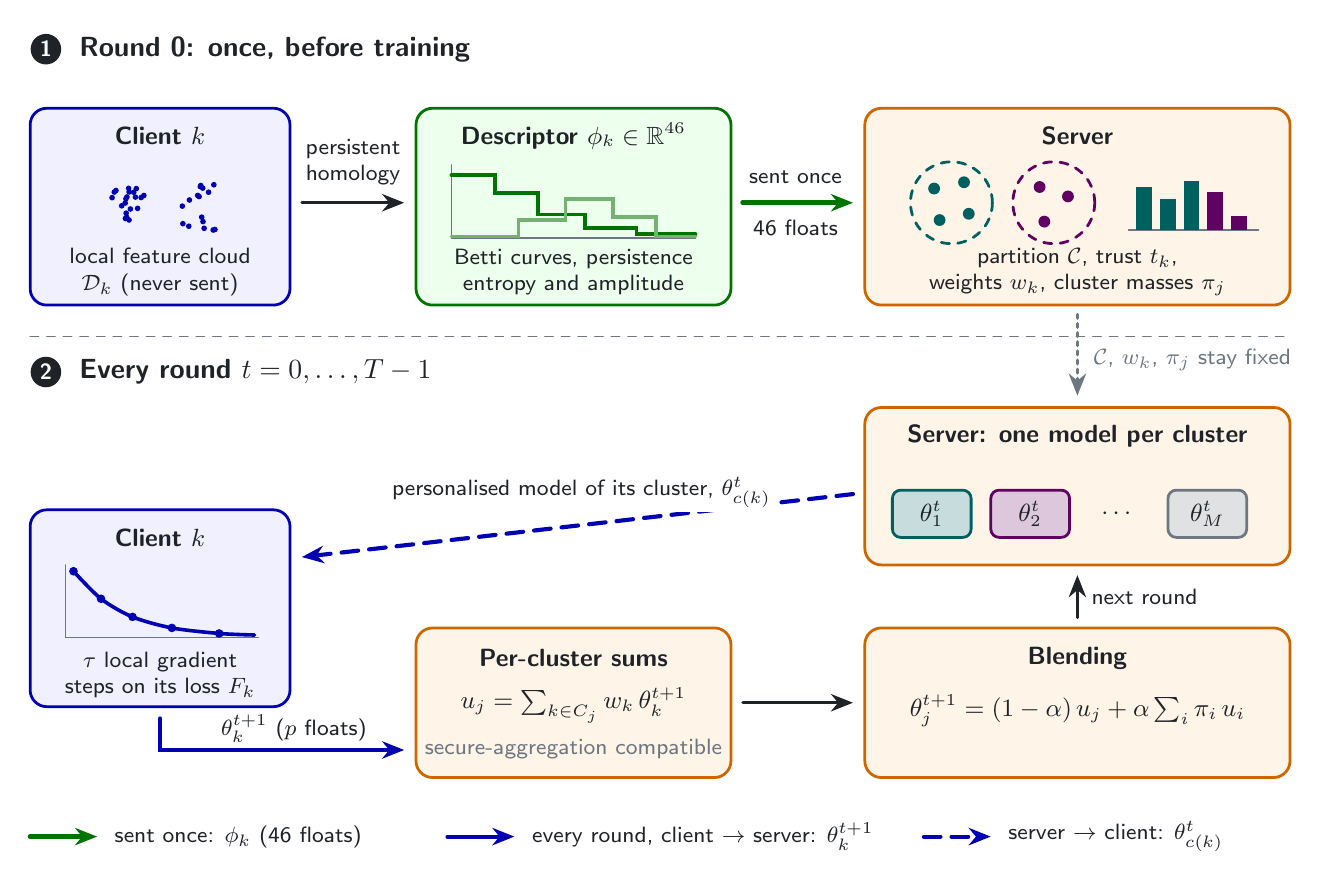
\begin{tikzpicture}[color=fg, font=\sffamily\small, line cap=round,
  >={Stealth[length=2.8mm,width=2.2mm]},
  box/.style={rounded corners=6pt, line width=1pt},
  head/.style={font=\sffamily\bfseries\small, text=fg},
  note/.style={font=\sffamily\footnotesize, text=fg, align=center},
  lab/.style={font=\sffamily\footnotesize, text=fg, fill=bg, inner sep=1.5pt, align=center},
  num/.style={circle, fill=fg, text=bg, inner sep=1.4pt, font=\sffamily\bfseries\footnotesize}]

% ============================ panel 1: round 0 ============================
\node[num] at (0.2,9.25) {1};
\node[anchor=west, font=\sffamily\bfseries\normalsize, text=fg] at (0.5,9.25) {Round 0: once, before training};

% client
\draw[box, draw=cl, fill=clfill] (0,6.0) rectangle (3.3,8.5);
\node[head] at (1.65,8.15) {Client $k$};
\pgfmathsetseed{11}
\foreach \i in {1,...,20} {\fill[cl] ({1.15+0.30*rand},{7.30+0.26*rand}) circle (0.036);}
\foreach \i in {1,...,16} {\fill[cl] ({2.15+0.22*rand},{7.25+0.32*rand}) circle (0.036);}
\node[note] at (1.65,6.42) {local feature cloud\\$\mathcal D_k$ (never sent)};

\draw[->, line width=1.1pt] (3.45,7.3) -- (4.75,7.3);
\node[note] at (4.1,7.82) {persistent\\homology};

% descriptor
\draw[box, draw=ds, fill=dsfill] (4.9,6.0) rectangle (8.9,8.5);
\node[head] at (6.9,8.15) {Descriptor $\phi_k\in\mathbb{R}^{46}$};
\draw[muted, line width=0.6pt] (5.35,6.85) -- (8.45,6.85);
\draw[muted, line width=0.6pt] (5.35,6.85) -- (5.35,7.78);
\draw[ds, line width=1.3pt] (5.35,7.65) -- (5.9,7.65) -- (5.9,7.42) -- (6.45,7.42) -- (6.45,7.15) -- (7.05,7.15)
      -- (7.05,6.98) -- (7.7,6.98) -- (7.7,6.9) -- (8.45,6.9);
\draw[ds!55!bg, line width=1.3pt] (5.35,6.87) -- (6.2,6.87) -- (6.2,7.08) -- (6.8,7.08) -- (6.8,7.35) -- (7.4,7.35)
      -- (7.4,7.12) -- (7.95,7.12) -- (7.95,6.87) -- (8.45,6.87);
\node[note] at (6.9,6.42) {Betti curves, persistence\\entropy and amplitude};

\draw[->, line width=1.8pt, draw=ds] (9.05,7.3) -- (10.45,7.3);
\node[lab] at (9.72,7.62) {sent once};
\node[lab] at (9.72,6.98) {46 floats};

% server structure
\draw[box, draw=sv, fill=svfill] (10.6,6.0) rectangle (16.0,8.5);
\node[head] at (13.3,8.15) {Server};
\draw[ca, dashed, line width=1pt] (11.7,7.3) circle (0.52);
\draw[cb, dashed, line width=1pt] (13.0,7.3) circle (0.52);
\foreach \p in {(11.48,7.48),(11.86,7.56),(11.55,7.08),(11.92,7.16)} \fill[ca] \p circle (0.075);
\foreach \p in {(12.82,7.5),(13.18,7.38),(12.88,7.06)} \fill[cb] \p circle (0.075);
\draw[muted, line width=0.6pt] (13.95,6.95) -- (15.6,6.95);
\foreach \x/\h/\c in {14.15/0.55/ca, 14.45/0.40/ca, 14.75/0.62/ca, 15.05/0.48/cb, 15.35/0.18/cb}
  \fill[\c] (\x-0.1,6.95) rectangle (\x+0.1,6.95+\h);
\node[note] at (13.3,6.42) {partition $\mathcal C$, trust $t_k$,\\weights $w_k$, cluster masses $\pi_j$};

% ============================ separator ============================
\draw[muted, dashed, line width=0.6pt] (0,5.6) -- (16,5.6);
\draw[->, muted, dotted, line width=1.3pt] (13.3,5.88) -- (13.3,4.85);
\node[lab, anchor=west, text=muted] at (13.45,5.3) {$\mathcal C$, $w_k$, $\pi_j$ stay fixed};

% ============================ panel 2: every round ============================
\node[num] at (0.2,5.15) {2};
\node[anchor=west, font=\sffamily\bfseries\normalsize, text=fg] at (0.5,5.15) {Every round $t=0,\dots,T-1$};

% server models
\draw[box, draw=sv, fill=svfill] (10.6,2.7) rectangle (16.0,4.7);
\node[head] at (13.3,4.33) {Server: one model per cluster};
\foreach \x/\c/\t in {11.45/ca/1, 12.7/cb/2, 14.95/muted/M}
  {\draw[\c, fill=\c!22!bg, rounded corners=3pt, line width=1pt] (\x-0.5,3.05) rectangle (\x+0.5,3.65);
   \node[text=fg] at (\x,3.35) {$\theta^{t}_{\t}$};}
\node[text=fg] at (13.82,3.35) {$\cdots$};

% client training
\draw[box, draw=cl, fill=clfill] (0,0.9) rectangle (3.3,3.4);
\node[head] at (1.65,3.05) {Client $k$};
\draw[muted, line width=0.6pt] (0.45,1.78) -- (2.9,1.78);
\draw[muted, line width=0.6pt] (0.45,1.78) -- (0.45,2.7);
\draw[cl, line width=1.3pt] plot[smooth] coordinates {(0.55,2.62) (0.9,2.27) (1.3,2.04) (1.8,1.9) (2.4,1.83) (2.85,1.81)};
\foreach \p in {(0.55,2.62),(0.9,2.27),(1.3,2.04),(1.8,1.9),(2.4,1.83)} \fill[cl] \p circle (0.055);
\node[note] at (1.65,1.3) {$\tau$ local gradient\\steps on its loss $F_k$};

% broadcast (dashed) and upload (solid)
\draw[->, line width=1.5pt, draw=cl, dash pattern=on 6pt off 4pt] (10.45,3.6) -- (3.45,2.8);
\node[lab] at (7.0,3.62) {personalised model of its cluster, $\theta^{t}_{c(k)}$};
\draw[->, line width=1.5pt, draw=cl] (1.65,0.75) |- (4.75,0.35);
\node[lab] at (3.35,0.62) {$\theta^{t+1}_k$ ($p$ floats)};

% aggregation and blending
\draw[box, draw=sv, fill=svfill] (4.9,0) rectangle (8.9,1.9);
\node[head] at (6.9,1.52) {Per-cluster sums};
\node[text=fg] at (6.9,0.92) {$u_j=\sum_{k\in C_j} w_k\,\theta^{t+1}_k$};
\node[note, text=muted] at (6.9,0.36) {secure-aggregation compatible};
\draw[->, line width=1.1pt] (9.05,0.95) -- (10.45,0.95);
\draw[box, draw=sv, fill=svfill] (10.6,0) rectangle (16.0,1.9);
\node[head] at (13.3,1.52) {Blending};
\node[text=fg] at (13.3,0.85) {$\theta^{t+1}_j=(1-\alpha)\,u_j+\alpha\sum_i\pi_i\,u_i$};
\draw[->, line width=1.1pt] (13.3,2.03) -- (13.3,2.57);
\node[lab, anchor=west] at (13.42,2.3) {next round};

% ============================ legend ============================
\draw[->, line width=1.8pt, draw=ds] (0,-0.75) -- (0.85,-0.75);
\node[anchor=west, font=\sffamily\footnotesize] at (0.95,-0.75) {sent once: $\phi_k$ (46 floats)};
\draw[->, line width=1.5pt, draw=cl] (5.3,-0.75) -- (6.15,-0.75);
\node[anchor=west, font=\sffamily\footnotesize] at (6.25,-0.75) {every round, client $\to$ server: $\theta^{t+1}_k$};
\draw[->, line width=1.5pt, draw=cl, dash pattern=on 6pt off 4pt] (11.35,-0.75) -- (12.2,-0.75);
\node[anchor=west, font=\sffamily\footnotesize] at (12.3,-0.75) {server $\to$ client: $\theta^{t}_{c(k)}$};
\end{tikzpicture}
\end{document}
